%%%%%%%%%%%%%%%%%%%%%%%%%%%%%%%%%%%%%%%%%
% Classicthesis Typographic Thesis
% LaTeX Template
% Version 1.3 (15/2/14)
%
% This template has been downloaded from:
% http://www.LaTeXTemplates.com
%
% Original author:
% André Miede (http://www.miede.de)
%
% License:
% CC BY-NC-SA 3.0 (http://creativecommons.org/licenses/by-nc-sa/3.0/)
%
% General Tips:
% 1) Make sure to edit the classicthesis-config.file
% 2) New enumeration (A., B., C., etc in small caps): \begin{aenumerate} \end{aenumerate}
% 3) For margin notes: \marginpar or \graffito{}
% 4) Do not use bold fonts in this style, it is designed around them
% 5) Use tables as in the examples
% 6) See classicthesis-preamble.sty for useful commands
%
%%%%%%%%%%%%%%%%%%%%%%%%%%%%%%%%%%%%%%%%%

%----------------------------------------------------------------------------------------
%	PACKAGES AND OTHER DOCUMENT CONFIGURATIONS
%----------------------------------------------------------------------------------------

\documentclass[
		twoside,openright,titlepage,numbers=noenddot,headinclude,%1headlines,
                footinclude=true,cleardoublepage=empty,
                BCOR=10mm,paper=a4,fontsize=12pt, % Binding correction, paper type and font size
                ngerman,british,brazilian, % Languages
                ]{scrreprt} 
                
% Includes the file which contains all the document configurations and packages - make sure to edit this file
%%%%%%%%%%%%%%%%%%%%%%%%%%%%%%%%%%%%%%%%%
% Thesis Configuration File
%
% The main lines to change in this file are in the DOCUMENT VARIABLES
% section, the rest of the file is for advanced configuration.
%
%%%%%%%%%%%%%%%%%%%%%%%%%%%%%%%%%%%%%%%%%

%----------------------------------------------------------------------------------------
%	DOCUMENT VARIABLES
%	Fill in the lines below to enter your information into the thesis template
%	Each of the commands can be cited anywhere in the thesis
%----------------------------------------------------------------------------------------

% Remove drafting to get rid of the '[ Date - classicthesis version 4.0 ]' text at the bottom of every page
\PassOptionsToPackage{eulerchapternumbers,listings, pdfspacing, subfig,beramono,parts,dottedtoc,linedheaders}{classicthesis}
% Available options: drafting parts nochapters linedheaders eulerchapternumbers beramono eulermath pdfspacing minionprospacing tocaligned dottedtoc manychapters listings floatperchapter subfig
% Adding 'dottedtoc' will make page numbers in the table of contents flushed right with dots leading to them

\newcommand{\myTitle}{Thesis Title\xspace}
%\newcommand{\mySubtitle}{An Homage to The Elements of Typographic Style\xspace}
\newcommand{\myDegree}{Master of Arts in International Relations\xspace}
\newcommand{\myName}{Danilo Alves Mendes Freire\xspace}
\newcommand{\myProf}{Professor Ravinder Bhavnani\xspace}
\newcommand{\myOtherProf}{Put name here\xspace}
\newcommand{\mySupervisor}{Put name here\xspace}
\newcommand{\myFaculty}{The Graduate Institute of International\\and Development Studies, Geneva\xspace}
\newcommand{\myDepartment}{Department of International Relations\xspace}
\newcommand{\myUni}{The Graduate Institute of International and Development Studies\xspace}
\newcommand{\myLocation}{Geneva\xspace}
\newcommand{\myTime}{June 2014\xspace}
%\newcommand{\myVersion}{version 4.0\xspace}

%----------------------------------------------------------------------------------------
%	USEFUL COMMANDS
%----------------------------------------------------------------------------------------

\newcommand{\ie}{i.\,e.}
\newcommand{\Ie}{I.\,e.}
\newcommand{\eg}{e.\,g.}
\newcommand{\Eg}{E.\,g.} 

\newcounter{dummy} % Necessary for correct hyperlinks (to index, bib, etc.)
\providecommand{\mLyX}{L\kern-.1667em\lower.25em\hbox{Y}\kern-.125emX\@}

%----------------------------------------------------------------------------------------
%	PACKAGES
%----------------------------------------------------------------------------------------
\makeatletter
\renewcommand{\@chapapp}{}% Not necessary...
\newenvironment{chapquote}[2][2em]
  {\setlength{\@tempdima}{#1}%
   \def\chapquote@author{#2}%
   \parshape 1 \@tempdima \dimexpr\textwidth-2\@tempdima\relax%
   \itshape}
  {\par\normalfont\hfill--\ \chapquote@author\hspace*{\@tempdima}\par\bigskip}
\makeatother
\usepackage{courier}

%------------------------------------------------

\exhyphenpenalty=1000
\hyphenpenalty=1000
\widowpenalty=1000
\clubpenalty=1000

%-------------------------------------------------
 
\PassOptionsToPackage{latin9}{inputenc} % latin9 (ISO-8859-9) = latin1+"Euro sign"
\usepackage{inputenc}
\usepackage{sidenotes} % allows sidenotes! Just type \sidenote{} to replace footnotes with sidenotes! My question here: http://tex.stackexchange.com/questions/163544/replacing-footnotes-with-sidenotes-in-classicthesis/
% the command for writing at the margins, without notes, is \marginpar{}

 
 %------------------------------------------------

%\PassOptionsToPackage{ngerman,american}{babel}  % Change this to your language(s)
% Spanish languages need extra options in order to work with this template
%\PassOptionsToPackage{spanish,es-lcroman}{babel}
\usepackage[british]{babel}

%------------------------------------------------			
\PassOptionsToPackage{round, sort&compress}{natbib}
\usepackage{natbib}
 
 %------------------------------------------------

%\PassOptionsToPackage{fleqn}{amsmath} % Math environments and more by the AMS 
\usepackage{amsmath, amsthm, amssymb, amsfonts}
 
 %------------------------------------------------

\PassOptionsToPackage{T1}{fontenc} % T2A for cyrillics
\usepackage{fontenc}

%------------------------------------------------

\usepackage{xspace} % To get the spacing after macros right

%------------------------------------------------

\usepackage{mparhack} % To get marginpar right

%------------------------------------------------

\usepackage{fixltx2e} % Fixes some LaTeX stuff 

%------------------------------------------------

\PassOptionsToPackage{smaller}{acronym} % Include printonlyused in the first bracket to only show acronyms used in the text
\usepackage{acronym} % nice macros for handling all acronyms in the thesis

%------------------------------------------------

%\renewcommand*{\acsfont}[1]{\textssc{#1}} % For MinionPro
\renewcommand{\bflabel}[1]{{#1}\hfill} % Fix the list of acronyms

%------------------------------------------------

\PassOptionsToPackage{pdftex}{graphicx}
\usepackage{graphicx} 

%----------------------------------------------------------------------------------------
%	FLOATS: TABLES, FIGURES AND CAPTIONS SETUP
%----------------------------------------------------------------------------------------

\usepackage{tabularx} % Better tables
\setlength{\extrarowheight}{3pt} % Increase table row height
\newcommand{\tableheadline}[1]{\multicolumn{1}{c}{\spacedlowsmallcaps{#1}}}
\newcommand{\myfloatalign}{\centering} % To be used with each float for alignment
\usepackage{caption}
\captionsetup{format=hang,font=small}
\usepackage{subfig}  

%----------------------------------------------------------------------------------------
%	CODE LISTINGS SETUP
%----------------------------------------------------------------------------------------

\usepackage{listings} 
%\lstset{emph={trueIndex,root},emphstyle=\color{BlueViolet}}%\underbar} % for special keywords
\lstset{language=[LaTeX]Tex, % Specify the language for listings here
keywordstyle=\color{RoyalBlue}, % Add \bfseries for bold
basicstyle=\small\ttfamily, % Makes listings a smaller font size and a different font
identifierstyle=\color{NavyBlue}, % Color of text inside brackets
commentstyle=\color{Green}\ttfamily, % Color of comments
stringstyle=\rmfamily, % Font type to use for strings
numbers=left, % Change left to none to remove line numbers
numberstyle=\scriptsize, % Font size of the line numbers
stepnumber=5, % Increment of line numbers
numbersep=8pt, % Distance of line numbers from code listing
showstringspaces=false, % Sets whether spaces in strings should appear underlined
breaklines=true, % Force the code to stay in the confines of the listing box
%frameround=ftff, % Uncomment for rounded frame
frame=single, % Frame border - none/leftline/topline/bottomline/lines/single/shadowbox/L
belowcaptionskip=.75\baselineskip % Space after the "Listing #: Desciption" text and the listing box
}

%----------------------------------------------------------------------------------------
%	HYPERREFERENCES
%----------------------------------------------------------------------------------------

\PassOptionsToPackage{pdftex,hyperfootnotes=false,pdfpagelabels}{hyperref}
\usepackage{hyperref}  % backref linktocpage pagebackref
\pdfcompresslevel=9
\pdfadjustspacing=1

\hypersetup{
% Uncomment the line below to remove all links (to references, figures, tables, etc)
%draft, 
colorlinks=true, linktocpage=true, pdfstartpage=3, pdfstartview=FitV,
% Uncomment the line below if you want to have black links (e.g. for printing black and white)
%colorlinks=false, linktocpage=false, pdfborder={0 0 0}, pdfstartpage=3, pdfstartview=FitV, 
breaklinks=true, pdfpagemode=UseNone, pageanchor=true, pdfpagemode=UseOutlines,
plainpages=false, bookmarksnumbered, bookmarksopen=true, bookmarksopenlevel=1,
hypertexnames=true, pdfhighlight=/O, urlcolor=NavyBlue, linkcolor=NavyBlue, citecolor=NavyBlue,
%------------------------------------------------
% PDF file meta-information
pdftitle={Entering the Underworld},
pdfauthor={Danilo Freire},
pdfsubject={},
pdfkeywords={Organised Crime, Prison Gangs, PCC, S\~{a}o Paulo, Brazil},
pdfcreator={pdfLaTeX},
pdfproducer={LaTeX with hyperref and classicthesis}
%------------------------------------------------
}   

%----------------------------------------------------------------------------------------
%	BACKREFERENCES
%----------------------------------------------------------------------------------------

\usepackage{ifthen} % Allows the user of the \ifthenelse command
\newboolean{enable-backrefs} % Variable to enable backrefs in the bibliography
\setboolean{enable-backrefs}{true} % Variable value: true or false

\newcommand{\backrefnotcitedstring}{\relax} % (Not cited.)
\newcommand{\backrefcitedsinglestring}[1]{Cited on page~#1.}
\newcommand{\backrefcitedmultistring}[1]{Cited on pages~#1.}
\ifthenelse{\boolean{enable-backrefs}} % If backrefs were enabled
{
\PassOptionsToPackage{hyperpageref}{backref}
\usepackage{backref} % to be loaded after hyperref package 
\renewcommand{\backreftwosep}{ and~} % separate 2 pages
\renewcommand{\backreflastsep}{, and~} % separate last of longer list
\renewcommand*{\backref}[1]{}  % disable standard
\renewcommand*{\backrefalt}[4]{% detailed backref
\ifcase #1 
\backrefnotcitedstring
\or
\backrefcitedsinglestring{#2}
\else
\backrefcitedmultistring{#2}
\fi}
}{\relax} 

%----------------------------------------------------------------------------------------
%	AUTOREFERENCES SETUP
%	Redefines how references in text are prefaced for different 
%	languages (e.g. "Section 1.2" or "section 1.2")
%----------------------------------------------------------------------------------------

\makeatletter
\@ifpackageloaded{babel}
{
\addto\extrasamerican{
\renewcommand*{\figureautorefname}{Figure}
%\renewcommand*{\tableautorefname}{Table}
\renewcommand*{\partautorefname}{Part}
\renewcommand*{\chapterautorefname}{Chapter}
\renewcommand*{\sectionautorefname}{Section}
\renewcommand*{\subsectionautorefname}{Section}
\renewcommand*{\subsubsectionautorefname}{Section}
}
\addto\extrasngerman{
\renewcommand*{\paragraphautorefname}{Absatz}
\renewcommand*{\subparagraphautorefname}{Unterabsatz}
\renewcommand*{\footnoteautorefname}{Fu\"snote}
\renewcommand*{\FancyVerbLineautorefname}{Zeile}
\renewcommand*{\theoremautorefname}{Theorem}
\renewcommand*{\appendixautorefname}{Anhang}
\renewcommand*{\equationautorefname}{Gleichung}
\renewcommand*{\itemautorefname}{Punkt}
}
\providecommand{\subfigureautorefname}{\figureautorefname} % Fix to getting autorefs for subfigures right
}{\relax}
\makeatother

%----------------------------------------------------------------------------------------

\usepackage[linedheaders]{classicthesis} 
\usepackage[left=3.5cm,right=3.5cm,top=3cm,bottom=3cm]{geometry}
%\areaset[current]{\dimexpr\textwidth+\marginparwidth+\marginparsep}{\textheight}
%\setlength{\marginparwidth}{0pt}
%\setlength{\marginparsep}{0pt}

%--------------------------------------------
\usepackage{setspace} 
\onehalfspacing
\usepackage{marginnote}

%----------------------ASMATH---------------
%\usepackage{amsmath}

%---------------------TIKZ------
\usepackage{tikz}
\usepackage[dvipsnames]{xcolor}
\usepackage{cleveref}
\usepackage{qtree}
\usepackage{tikz-qtree}
\usetikzlibrary{calc}
\usetikzlibrary{positioning}
%----------------------------------------------------------------------------------------
%	CHANGING TEXT AREA 
%----------------------------------------------------------------------------------------

%\linespread{1.05} % a bit more for Palatino
%\areaset[current]{312pt}{761pt} % 686 (factor 2.2) + 33 head + 42 head \the\footskip
%\setlength{\marginparwidth}{7em}%
%\setlength{\marginparsep}{2em}%

%----------------------------------------------------------------------------------------
%	USING DIFFERENT FONTS
%----------------------------------------------------------------------------------------

\usepackage[oldstylenums]{kpfonts} % oldstyle notextcomp
%\usepackage[osf]{libertine}
%\usepackage{hfoldsty} % Computer Modern with osf
%\usepackage[light,condensed,math]{iwona}
%\renewcommand{\sfdefault}{iwona}
%\usepackage{lmodern} % <-- no osf support :-(
%\usepackage[urw-garamond]{mathdesign} <-- no osf support :-(

\begin{document}

%\frenchspacing % Reduces space after periods to make text more compact

\raggedbottom % Makes all pages the height of the text on that page

\selectlanguage{british} % Select your default language - e.g. american or ngerman

%\renewcommand*{\bibname}{new name} % Uncomment to change the name of the bibliography
%\setbibpreamble{} % Uncomment to include a preamble to the bibliography - some text before the reference list starts

\pagenumbering{roman} % Roman page numbering prior to the start of the thesis content (i, ii, iii, etc)

\pagestyle{plain} % Suppress headers for the pre-content pages

\setlength{\cftbeforechapskip}{0.5em} % change vertical skip before chapters


%----------------------------------------------------------------------------------------
%	PRE-CONTENT THESIS PAGES
%----------------------------------------------------------------------------------------

% Title Page

%\begin{titlepage}

%\begin{addmargin}[-1cm]{-3cm}
% \begin{center}
% \large

% \hfill
% \vfill

% \begingroup
% \color{Maroon}\spacedallcaps{\myTitle} \\ \bigskip % Thesis title
% \endgroup

% \spacedlowsmallcaps{\myName} % Your name

% \vfill

%\includegraphics[width=6cm]{gfx/TFZsuperellipse_bw} \\ \medskip % Picture

%\mySubtitle \\ \medskip % Thesis subtitle
%\myDegree \\
% \myFaculty \\
% \myDepartment \\
%\myUni \\ 
% \bigskip

% \myTime\ %-- \myVersion % Time and version

% \vfill

% \end{center}
%\end{addmargin}

% \end{titlepage}

%##############################

\begin{titlepage}
\begin{flushleft}
	
\includegraphics[width=7cm]{gfx/logo.png}
\end{flushleft}
\vspace{4cm}
\begin{center}
	\begin{large}
		\textbf{Entering the Underworld: Prison Gang Recruitment\\ in S\~{a}o Paulo's Primeiro Comando da Capital}\\
	\end{large}
	\vspace{3cm}
	\begin{large}
		\textbf{DISSERTATION}\\
	\end{large}
	Submitted in fulfilment of the requirement for the \\
	Master in International Relations / Political Science (MIRPS)\\
	\vspace{2cm}
	by \\
	Danilo Alves Mendes Freire\\
	(Brazil)\\
	\vspace{1.5cm}
	Geneva \\
	2014
\end{center}
\end{titlepage} % Main title page

% Back of the title page

\thispagestyle{empty}

\hfill

\vfill

\noindent\myName: \textit{Entering the Underworld: Prison Gang Recruitment in S\~{a}o Paulo's Primeiro Comando da Capital}. \myDegree, \myUni, \myLocation, \myTime.

% You may wish to do something with the back of the title page, such as including your supervisors, location or time frame of the work. Below is an example of doing so although you may want to tweak it to your liking.

\bigskip

\noindent\spacedlowsmallcaps{Supervisor}: \\
\myProf \\
%\myOtherProf \\ 
%\mySupervisor

\medskip

\noindent\spacedlowsmallcaps{Location}: \\
Geneva, Switzerland

\medskip

%\noindent\spacedlowsmallcaps{Time Frame}: \\
%\myTime
 % Back of the title page

%\cleardoublepage% Declaration

\refstepcounter{dummy}
\pdfbookmark[0]{Declaration}{declaration} % Bookmark name visible in a PDF viewer

\chapter*{Declaration} % Declaration section text

\thispagestyle{empty}

 
I hereby declare that

\begin{enumerate}
\item except where due acknowledgement has been made, the work is that of the author alone;
\item the work has not been submitted previously, in whole or in part, to qualify for any other academic award;
\item the content of the thesis is the result of work which has been carried out since the official commencement date of the approved research program;
\item any editorial work, paid or unpaid, carried out by a third party is acknowledged;
\item ethics procedures and guidelines have been followed.
\end{enumerate}

\bigskip
 
%\noindent\textit{\myLocation, \myTime}

\smallskip

\begin{flushright}
\begin{tabular}{m{6cm}}
\\ \hline
\centering Danilo Alves Mendes Freire\\Geneva, 16th June 2014
\end{tabular}
\end{flushright}
 % Declaration

\cleardoublepage% Dedication

\thispagestyle{empty}
\refstepcounter{dummy}

\pdfbookmark[1]{Dedication}{Dedication} % Bookmark name visible in a PDF viewer

\vspace*{3cm}

%\begin{center}
%\emph{Ohana} means family. \\
%Family means nobody gets left behind, or forgotten. \\ \medskip
%--- Lilo \& Stitch    
%\end{center}

\medskip

\begin{center}
Para Rosali Alves, minha m\~{a}e. \\ \smallskip
%1939\,--\,2005
\end{center} % Dedication page

%\cleardoublepage\include{FrontBackMatter/Foreword} % Uncomment and create a Foreword.tex to include a foreword

\cleardoublepage% Abstract

\pdfbookmark[1]{Abstract}{Abstract} % Bookmark name visible in a PDF viewer

\begingroup
\let\clearpage\relax
\let\cleardoublepage\relax
\let\cleardoublepage\relax

\chapter*{Abstract} % Abstract name

The present thesis provides a throughout discussion of the emergence of the \textit{Primeiro Comando da Capital} (PCC), a prison gang based in S\~{a}o Paulo, Brazil. Its main goal is to analyse how this criminal group selects its potential members. The work starts with a review of the recent literature on prison culture and gangs, with special emphasis on the Brazilian contributions to the field. Then it presents the first historical account of the PCC in the English language since previous research has been solely conducted in Portuguese. Lastly, the thesis offers a simple game-theoretical model to analyse both the incentives for a criminal to join a prison gang and how the PCC has been able to hire competent criminals under conditions of uncertainty and information asymmetry. The model suggest three findings. First, it stresses the role of informers in the gang's recruitment process. Informers allow the prison gang to keep a lower entry cost, so the gang can attract a larger pool of applicants and still be able to select competent candidates. Second, it indicates that 
there are cases in which joining a prison gang is not the best option for an inmate. When the detainee has enough skills to endure prison conditions by himself, the prisoner might be better off if he decides to ``go it alone'' and devote his ability exclusively to his own survival. Third, the models confirms the idea that the prison gang is not only a ``school of crime'', but perhaps most importantly, a highly effective screening device. Prison gangs increase the welfare of the inmates by providing an extremely valuable public good: reliable information. Public policies implications and possible extensions of the current study are also discussed.\\



%This criminal group, which currently extends its influence to around 90\% of its native state's penal system, was able to monopolise power in prisons by having only 3\% of the inmate population in its ranks. In the present work I develop a formal model to address this question and derive a few conclusion from it.

\noindent
\textsc{Keywords:} Organised Crime, Prison Gangs, PCC, S\~{a}o Paulo, Game Theory

\endgroup			

\vfill % Abstract page

\cleardoublepage% Acknowledgements

\pdfbookmark[1]{Acknowledgements}{Acknowledgements} % Bookmark name visible in a PDF viewer

%\singlespacing
%{\slshape  
%All human behaviour is scheduled and programmed through rationality. There is a logic of institutions and in behaviour and in political relations. In even the most violent ones there is a rationality. What is most dangerous in violence is its rationality. Of course violence itself is terrible. But the deepest root of violence and its permanence come out of the form of the rationality we use. The idea had been that if we live in the world of reason, we can get rid of violence. This is quite wrong. Between violence and rationality there is no incompatibility.} \\ \medskip
%--- Michel Foucault, \textit{Truth is in the Future}, p. 299.


\bigskip

%----------------------------------------------------------------------------------------

\begingroup

\let\clearpage\relax
\let\cleardoublepage\relax
\let\cleardoublepage\relax

\chapter*{Acknowledgements} % Acknowledgements section text
There are a number of people to whom I have to express my most sincere appreciation. First and foremost, I would like to convey my gratitude to my supervisor, Professor Ravi Bhavnani, for his guidance and support over the last two years. His contributions are felt throughout the text. I also thank Professor C\'{e}dric Dupont for being the second reader of this thesis.

Several people generously provided comments on this work. I owe thanks to Guilherme Arbache, Fabio Barros, Gustavo Burgos, Guilherme Duarte, Manoel Galdino, Le\^{o}ncio Junior, Sam Keb, Eben Kuni, Davi Moreira, Rafael Nunes, Pietro Rodrigues, Luis Felipe Serrao, Damien Someil, and Sabine Waltraut for their valuable contributions. My friend Umberto Mignozzetti deserves a special mention. Not only he helped me to translate my ideas into proper mathematics, but also made many insightful suggestions to  this dissertation. I am glad to have written my first academic papers with such a brilliant co-author, and I hope we continue to work together for many years. Of course, all faults remain my own.

I have benefited immensely from the help of many members of the open source software communities I am proud to be part of. Thanks to all those who anonymously answered my questions about computer programming, \LaTeX, \texttt{R}, and statistics on R-help and Stack Overflow. 

I also thank to my flatmates Kamel Belmkadden, Raquel Ermida, Jo\~{a}o Matos and Carlos Montesinos for the great time we had together in Geneva.

Guilherme Kerr, Gustavo Kerr and Mauricio Pantale\~{a}o, old brothers in arms, have always stood by my side in good and bad moments. This time it was no different. Thank you very much for the camaraderie. 

No acknowledgement would be complete without giving thanks to my dear Mira. She spent countless nights helping me to clarify my ideas and was always my support when there was no one to answer my queries. Vielen herzlichen Dank, Mimi.

Last but not least, my family has given me all support I needed to pursuit this project. My deepest thanks to my mother Rosali and my grandmother Maria for their unending trust, patience and love. De cora\c{c}\~{a}o, muito obrigado por tudo. Amo voc\^{e}s.



%Put your acknowledgements here.\\

%\noindent Many thanks to everybody who already sent me a postcard!\\

%\noindent Regarding the typography and other help, many thanks go to Marco Kuhlmann, Philipp Lehman, Lothar Schlesier, Jim Young, Lorenzo Pantieri and Enrico Gregorio\footnote{Members of GuIT (Gruppo Italiano Utilizzatori di \TeX\ e \LaTeX )}, J\"org Sommer, Joachim K\"ostler, Daniel Gottschlag, Denis Aydin, Paride Legovini, Steffen Prochnow, Nicolas Repp, Hinrich Harms, Roland Winkler,  and the whole \LaTeX-community for support, ideas and some great software.

%\bigskip

%\noindent\emph{Regarding \mLyX}: The \mLyX\ port was intially done by
%\emph{Nicholas Mariette} in March 2009 and continued by
%\emph{Ivo Pletikosi\'c} in 2011. Thank you very much for your work and the contributions to the original style.

\endgroup % Acknowledgements page

\pagestyle{scrheadings} % Show chapter titles as headings

\cleardoublepage% Table of Contents - List of Tables/Figures/Listings and Acronyms

\refstepcounter{dummy}

\pdfbookmark[1]{\contentsname}{tableofcontents} % Bookmark name visible in a PDF viewer

\setcounter{tocdepth}{2} % Depth of sections to include in the table of contents - currently up to subsections

\setcounter{secnumdepth}{3} % Depth of sections to number in the text itself - currently up to subsubsections

\manualmark
\markboth{\spacedlowsmallcaps{\contentsname}}{\spacedlowsmallcaps{\contentsname}}
\tableofcontents 
\automark[section]{chapter}
\renewcommand{\chaptermark}[1]{\markboth{\spacedlowsmallcaps{#1}}{\spacedlowsmallcaps{#1}}}
\renewcommand{\sectionmark}[1]{\markright{\thesection\enspace\spacedlowsmallcaps{#1}}}

\clearpage

\begingroup 
\let\clearpage\relax
\let\cleardoublepage\relax
\let\cleardoublepage\relax


%----------------------------------------------------------------------------------------
%	List of Figures
%----------------------------------------------------------------------------------------

\refstepcounter{dummy}
\addcontentsline{toc}{chapter}{\listfigurename} % Uncomment if you would like the list of figures to appear in the table of contents
\pdfbookmark[1]{\listfigurename}{lof} % Bookmark name visible in a PDF viewer
\label{sec:figures}
\listoffigures

\vspace*{8ex}
\newpage

%----------------------------------------------------------------------------------------
%	List of Tables
%----------------------------------------------------------------------------------------

%\refstepcounter{dummy}
%\addcontentsline{toc}{chapter}{\listtablename} % Uncomment if you would like the list of tables to appear in the table of contents
%\pdfbookmark[1]{\listtablename}{lot} % Bookmark name visible in a PDF viewer
%\label{sec:tables}
%\listoftables
        
%\vspace*{8ex}
%\newpage
    
%----------------------------------------------------------------------------------------
%	Acronyms
%----------------------------------------------------------------------------------------

\refstepcounter{dummy}
\addcontentsline{toc}{chapter}{Acronyms} % Uncomment if you would like the acronyms to appear in the table of contents
\pdfbookmark[1]{Acronyms}{acronyms} % Bookmark name visible in a PDF viewer
\label{sec:acronyms}
\markboth{\spacedlowsmallcaps{Acronyms}}{\spacedlowsmallcaps{Acronyms}}

\chapter*{Acronyms}

\begin{acronym}[UML]
\acro{CD}{Casa de Deten\c{c}\~{a}o de S\~{a}o Paulo (S\~{a}o Paulo Detention House)}
\acro{CV}{Comando Vermelho (Red Command)}
\acro{MDB}{Movimento Democr\'{a}tico Brasileiro (Brazilian Democratic Movement)}
\acro{PCC}{Primeiro Comando da Capital (First Command of the Capital)}
\acro{SAP}{Secretaria de Administra\c{c}\~{a}o Penitenci\'{a}ria (Secretary of Prison Administration)}
\acro{SSP}{Secretaria de Seguran\c{c}a P\'{u}blica (Secretary of Public Security)}
\end{acronym}  
                   
\endgroup % Contents, list of figures/tables/listings and acronyms

\cleardoublepage

\pagenumbering{arabic} % Arabic page numbering for thesis content (1, 2, 3, etc)
%\setcounter{page}{90} % Uncomment to manually start the page counter at an arbitrary value (for example if you wish to count the pre-content pages in the page count)

\cleardoublepage % Avoids problems with pdfbookmark

%----------------------------------------------------------------------------------------
%	THESIS CONTENT - CHAPTERS
%----------------------------------------------------------------------------------------

\ctparttext{The purpose of the following part is threefold. In the first chapter I introduce the thesis' main subject, the \textit{Primeiro Comando da Capital} (PCC), a prison gang based in S\~{a}o Paulo, Brazil, and discuss the puzzle that motivated this work. Later I review the recent literature on prison culture and gangs, emphasising the Brazilian contributions to the field. Then I present a history of the PCC, which will provide subsidies for the formal model to be developed in the second part.} % Text on the Part 1 page describing  the content in Part 1

\part{PCC: Theory and History} % First part of the thesis

\chapter{Introduction}
\label{ch:chap1}

%----------------------------------------------------------------------------------------

\begin{chapquote}{Michel Foucault, \textit{The Truth is in the Future}.}
All human behaviour is scheduled and programmed through rationality. There is a logic of institutions and in behaviour and in political relations. In even the most violent ones there is a rationality. What is most dangerous in violence is its rationality. Of course violence itself is terrible. But the deepest root of violence and its permanence come out of the form of the rationality we use. The idea had been that if we live in the world of reason, we can get rid of violence. This is quite wrong. Between violence and rationality there is no incompatibility.
\end{chapquote}

On 18th February 2001, Brazil's richest state was brought to a halt. In one ordinary Sunday afternoon, the \textit{Primeiro Comando da Capital}\footnote{Portuguese for ``First Command of the Capital'', the capital being the city of S\~{a}o Paulo. All abbreviations mentioned in this text, alongside their respective translations into English, are listed on page \pageref{sec:acronyms}.} (PCC hereafter) unexpectedly challenged the government forces and took over 29 prisons across the state of S\~{a}o Paulo \citep[208]{biondi2007relacoes}. According to official estimates, about 25,000 prisoners joined the rebellion, and in a single penitentiary, 8,000 inmates held more than 7,000 civilians as hostages, amongst them 1,750 children \citep[]{terra2001rebeliao}. The convicts protested against the transference of PCC leaders from the capital to the countryside. To organise what became known as ``the megarebellion'', they had been using smuggled mobile phones \citep[]{montandon2012sistema}. Heavily-armed government troops later stormed the prisons, and after hours of negotiations and the eventual use of lethal force (5 inmates were killed), the criminal organisation was finally contained. Nevertheless, the damage to the government's reputation had already been done. It was clear to everyone -- the media, public officials, citizens -- that the PCC was a social force not to be ignored. As summarised by \citet[387]{amorim2003cv}, in 2001, the PCC ``[\dots] publicly declared their hegemony over the prison system in S\~{a}o Paulo. A hegemony backed up by the magnitude of the rebellion itself [\dots].'' 

Five years later, the PCC performed yet another show of force. Between May and June 2006, the \textit{Comando} organised a series of attacks in no less than 82 prisons, 10 of them in other states. The violence also spread outside the prison walls. According to the Secretary of Public Security (SSP), PCC-affiliated members burned 82 buses, bombed 17 bank branches, killed 46 and wounded 78 police officers and penitentiary agents in 280 attacks to public buildings in the city of S\~{a}o Paulo alone \citep[]{folha2006rebeliao, terra2008rebeliao}. 

\begin{center}
\begin{figure}[bth]
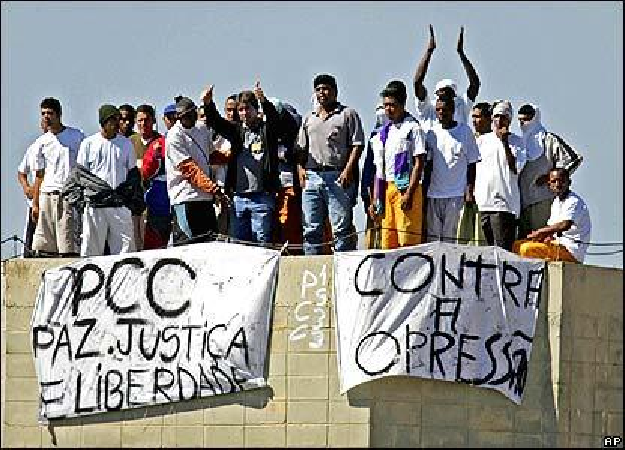
\includegraphics[height = 8cm, width = 1\linewidth]{gfx/fig1}
\caption[PCC Rebellion in 2006]{PCC Rebellion in 2006\footnotemark}
\label{fig:fig1}
\end{figure}
\end{center}

\footnotetext{Source: Associated Press. The banners read ``PCC, peace, justice and freedom'', and ``against oppression''. Regarding the 1533 written on the wall, the letter P is the 15th and C is the 3rd in the Brazilian alphabet, whereby 1533 means PCC. Except otherwise noted, all translations from Portuguese to English are my own.} The two rebellions have led to heated debates about the role of prison reform in the society \citep[323]{dias2009guerra}. Brazil's incarcerated population has skyrocketed in the last decades, and S\~{a}o Paulo provides perhaps the best example of such steady increase. The country currently has the fourth largest incarceration population in the world with around 574,000 prisoners\footnote{This number is only smaller than those of the United States (2.2 million inmates), China (1.6 million) and Russia (740,000) \citep{agenciabrasil2014prisaobrasil}.}. S\~{a}o Paulo alone holds around 200,000 convicts (35\% of the total) and adds another 15,000 inmates to the official statistics every year \citep{brasildefato2013numeropresos}. The trend can be seen in \autoref{fig:fig2} below. The massive growth in incarceration rates has created serious problems to the Brazilian prison system: overcrowding, staff shortage, and inadequate legal services, sanitation and health care present in virtually every penitentiary of the country \citep[275]{darke2013inmate}.

\begin{center}
\begin{figure}[bth]
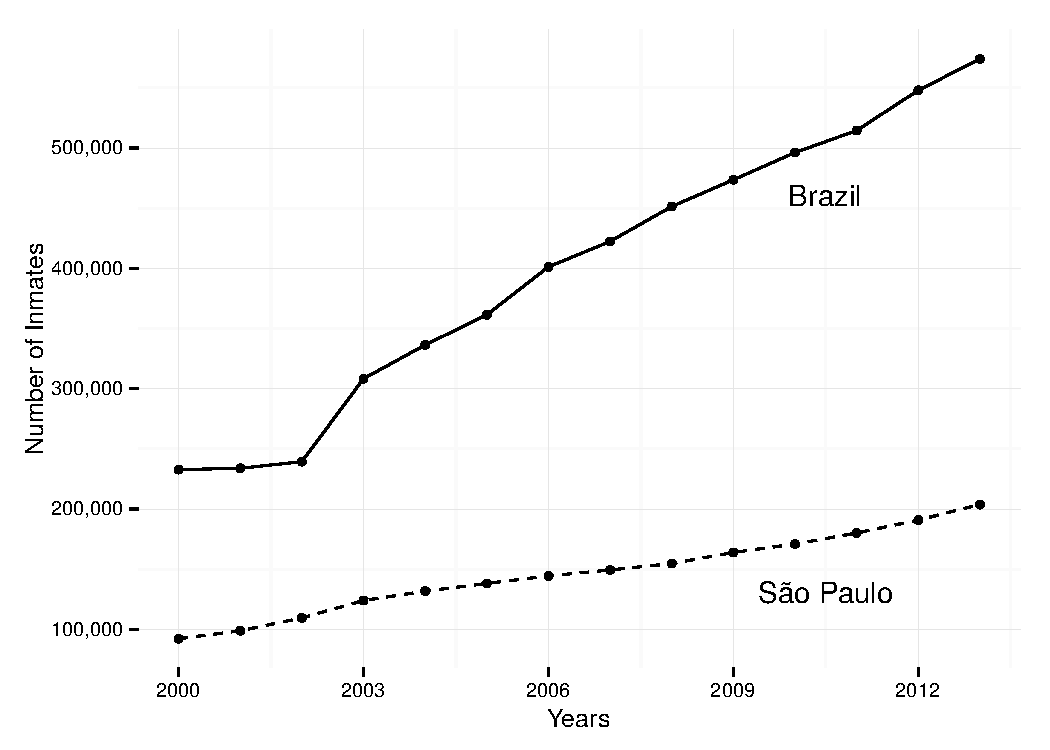
\includegraphics[height = 8cm, width = 1\linewidth]{gfx/fig2}
\caption[Prison Population (2000--2013)]{Prison Population (2000--2013)\footnotemark}
\label{fig:fig2}
\end{figure}
\end{center}

\footnotetext{Source: Own authorship with data provided by the Brazilian Ministry of Justice. Stable links: \href{http://bit.ly/1rImlPE}{http://bit.ly/1rImlPE} and \href{http://bit.ly/1ixhY8z}{http://bit.ly/1ixhY8z} [Access: 23th April 2014]. All graphs displayed in this thesis were created with \texttt{R} statistical language version 3.1.0 \citep{rstats} and the \texttt{ggplot2} package version 0.9.3.1 \citep{ggplot2}. Reproducible code for the figures are included in the \autoref{sec:appendix}.} Furthermore, as in other parts of the country \citep{zaluar1999debate}, the vast majority of prisoners in S\~{a}o Paulo are black and from low social strata \citep[16]{adorno2007organized}, groups with few economic opportunities apart from those offered by illicit markets\footnote{Brazil was a slave country until 1889, and racial prejudice has never been absent in the country. While blacks currently comprise 51\% of the Brazilian population \citep{secretariaassuntos2012populacaonegra}, they make 66\% of homicide victims and 65\% of the total number of convicts in the country \citep{waiselfisz2012mapa}. As described by \citet[1]{adorno1996racismo}, ``[\dots] crime is not exclusive to the black population, but punishment seems to be.''}. In this regard, prison gangs are not only important for protection, but also for being able to reduce the ``income loss'' suffered by an individual if he is put behind bars. The PCC was explicitly structured around this principle: its internal statute clearly declares that ``[\dots] those who are in liberty [should contribute] to the brothers inside prisons [PCC members] through lawyers, money, help to family members and prison outbreak operations'' \citep{folha2001estatutopcc}. By giving economic incentives to other inmates, the PCC can expand their cadres and increase the general welfare of the inmates. In a region where inequality is rampant and the state has thus far failed to properly address the issue of poverty \citep{chiavegatto2012cause, marques2012opportunities}, the fact that the PCC currently provides food supplies, financial assistance, medicines, private health care, and legal advice \citep{defesanet2012estatutopcc} makes the organisation notably attractive for a large number of inmates. 

It has also been noted that the PCC significantly contributed to the reduction in violence within S\~{a}o Paulo's prison system. At least since the mid-2000s, the group has been able to emerge as an undisputed mediator and solve conflicts between inmates. \citet[83]{dias2009ocupando} affirms that ``[\dots] when unable to constitute a universal source of regulation, the official law leaves gaps which are filled by informal instances -- such as the Primeiro Comando da Capital (PCC), in the prisons of S\~{a}o Paulo.'' The gang has implemented informal courts that resemble state institutions, and those ``debates'' -- how such illegal tribunals are called\footnote{The original term is spelt the same way in Portuguese, \textit{debates} \citep[3]{feltran2012metodos}.} -- have progressively replaced other forms of ``popular justice'' such as lynchings and hiring of target killers \citep[3]{feltran2012metodos}. Moreover, the \textit{Comando} has developed a series of assertive ways to verbally terrorise inmates. Since the PCC's threats are credible, such meetings with actual or potential undisciplined members are effective deterrence factors\footnote{The practice is known within and outside PCC circles as \textit{dar um psicol\'{o}gico}, ``to put psychological [pressure]'' \citep{marques2010liderancca}.}.

The rise of the PCC has also brought other positive changes to public security. The city of S\~{a}o Paulo, capital of the state of the same name, was knowingly one of the most violent places in the world. Nevertheless, S\~{a}o Paulo has experienced a drastic reduction in homicides over the past years. A number of authors argue that the establishment of the PCC as the city's (and the state's) major drug gang has accounted for most of the decline in murders in the metropolis. \cite{biondi2010junto} and \cite{dias2011pulverizaccao}, for instance, note that the PCC has instituted a policy that explicitly forbids the use of lethal violence as a means to settle disputes between members and severely punishes those who refuse to abide by that rule \citep{jozino2004cobras}. Since poor young males have the highest risk of being both victims of murder in S\~{a}o Paulo and members of the PCC, the correlation between the emergence of the cartel and the drop in homicide rates seems plausible. \autoref{fig:fig3} shows the evolution of murder rates in the city of S\~{a}o Paulo. 


%From 2000 to 2007, the number of murders declined from 5,979 to 1,311 (-78\%), and S\~{a}o Paulo's poorest districts have seen even larger declines in murder rates. Homicides in Cap\~{a}o Redondo declined from 203 in 2002 to 23 in 2007; in Itaquera, from 140 in 2001 to 20 in 2007; in Cidade Tiradentes, from 195 in 2000 to 24 in 2007; and in Jardim \^{A}ngela there were 53 homicides in 2007, down from 277 in 2001. 

\begin{center}
\begin{figure}[bth!]
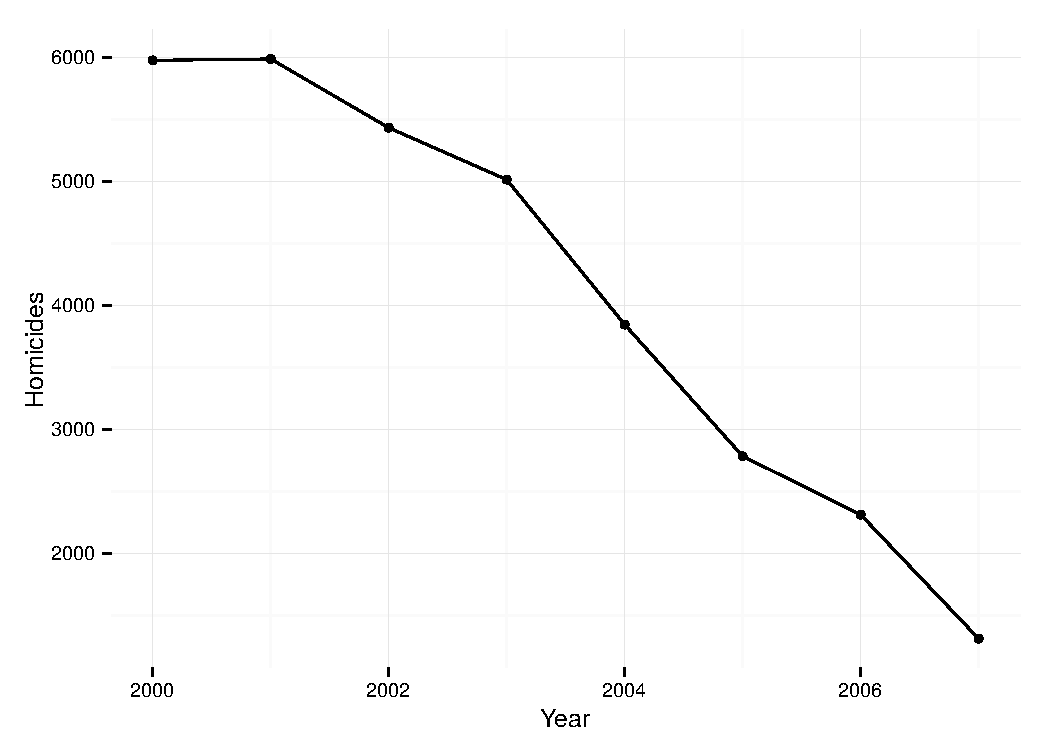
\includegraphics[height = 8cm, width = 1\linewidth]{gfx/fig3}
\caption[Homicides in S\~{a}o Paulo (2000--2007)]{Homicides in S\~{a}o Paulo (2000--2007)\footnotemark}
\label{fig:fig3}
\end{figure}
\end{center}

\footnotetext{Source: Own authorship. Data collected by the Centre for the Study of Violence at the University of S\~{a}o Paulo. Stable link: \href{http://bit.ly/Sg7qjB}{http://bit.ly/Sg7qjB} [Access: 24th March 2014].} %The reduction of violence in poor areas have also lent legitimacy to the PCC. The cartel can now enjoy greater support from the extended families of the inmates, many of them who directly benefited from the lowering of homicide rates \citep{feltran2008legitimo, feltran2012metodos}.

Curiously, the PCC has managed to accomplish all those goals while representing \textit{less than 3\%} of S\~{a}o Paulo's inmate population \citep[]{bbc2013pcc, veja2013crescimentopcc}. The task is indeed impressive if one keeps in mind that criminals face enormous challenges when trying to provide private governance \citep{sheptycki2003governance}. Given the constant fear of being arrested by the police \citep{williams2002cooperation}, criminals encounter several problems to identify their peers and communicate with each other \citep[xii]{gambetta2009codes}. Also, as a result of the inherently violent nature of many illegal activities, attempts to establish bonds of trust between criminals are rare and likely to fail \citep{liebling2012social, von2004organized}. Due to these obstacles, criminal networks are an intriguing object of study for those interested in cooperation issues and the role of violence, incentives and signals as credible commitments in social groups \citep{campana2013cooperation, densley2012street, freeman1994crime}.

This poses two clear questions that so far have not been addressed by the specialised literature on the PCC. First, why is not \textit{every} detainee a PCC member? Since the PCC is able to considerably ameliorate prison conditions, why would someone prefer \textit{not} to join the gang? ``Going alone'' seems to be an irrational strategy to all inmates, so why would they adopt it? Second, how can the PCC find a ``competent'' criminal to join its ranks in such a violent, uncertain environment as the prison? As any other organisation or firm, the PCC knows that ``qualified candidates'' are a scarce resource, and the group wants to select qualified mobsters and reject bad ones. But how can the gang do so if criminals have strong incentives to hide their intentions and lie about their skills? 

%Given the clear importance of the PCC in Brazil's current history, it is surprising that the topic has attracted such a limited number of researchers. \citet[365]{dias2011pulverizaccao} notes that while there is a significant number of writings focused on the judicial dimension of organised crime, the literature analysing empirical aspects of criminal institutions is still comparatively small. Apart from a few books written by investigative journalists \citep{amorim2003cv, jozino2004cobras, souza2007pcc}, and some fieldwork studies produced by anthropologists and sociologists \citep{biondi2010junto, dias2009guerra, dias2011pulverizaccao, marques2010liderancca}, no analytical work has ever been written on the group. In this sense, political scientists could contribute to this debate not only by offering a more general theory derived from the findings presented in the literature, but also by using techniques which have so not been employed to analyse the organised crime in S\~{a}o Paulo. 

In the present thesis, I develop a formal model to address these  lacunae in the recent literature. Game theory is a useful tool to evaluate deductive logic and test causal mechanisms, specially in situations where first-hand information is either unavailable or too risky to obtain. However, while those methods are now widely employed in international relations and comparative politics  \citep[e.g.][]{de1999institutional, fearon1995rationalist, mccarty2007political}, their use is still notably limited in criminal studies. With noteworthy exceptions \citep[]{dixit2011game, lessing2014cddrl}, formal theorists have so far largely ignored prison gangs. With regards to the PCC, there is not a single study that uses formal modelling to evaluate the operations of the cartel, even though some of the topics related to the organisation could be translated into mathematical terms. This work aims to partially fill this gap.

In \autoref{ch:chap2} I offer a brief review of the recent literature on prison culture and gangs, emphasising the Brazilian contributions to the topic. \hyperlink{page.19}{Chapter 3} presents a short history of the Primeiro Comando da Capital, which to the best of my knowledge has not yet been published in the English language. In \autoref{ch:chap4} I develop a simple formal model discussing under what condition inmates would decide to join the criminal organisation and how the PCC is able to successfully select potential candidates. Based upon the rational theory of crime and on qualitative evidence, I intend to present a general framework to understand the problems of individual choice regarding a criminal organisation, and decision-making under conditions of extreme uncertainty. Both analyses are knowingly modest, but they represent new contributions to the field.

%% Comment this last paragraph


% \citep[e.g.][]{bhavnani2006ethnic, bhavnani2000localized, de1999institutional, epstein2002modeling, mccarty2007political}
 % Chapter 1
\chapter{Literature Review}
\label{ch:chap2} 

%------------------------------------------------------------------------------

\begin{chapquote}{Jos\'{e} Saramago, \textit{The Double}.}
Chaos is merely order waiting to be deciphered.
\end{chapquote}

Scholars have long been interested in the culture of prisons \citep[398]{hunt1993changes}. As other subjects in modern sociology and political science \citep[]{hoffmann2000american, munck2008passion}, prison studies started as a mainly American discipline. Therefore, this chapter begins with a brief discussion on the American literature on prison culture and gangs, followed by a review of recent texts on the PCC, largely written in Brazil and so far accessible only in Portuguese. 

\section{Theoretical Models of Prison Behaviour}

The study of inmate culture can be traced back to the 1940s \citep[]{glaser1972bibliography} when \cite{clemmer1940prison} published his pioneer work on inmate life in a maximum security prison in the United States. The author argued that inmate behaviour is a function of the prison environment, and that this structural condition determines inmates' attitudes and mores \citep[62]{craddock1996comparative}. An important concept formulated by \citet[270]{clemmer1940prison} is \textit{prisonisation}, which describes the fact that inmates progressively adopt the subculture of prisons, itself established in order to cope with the difficulties of being incarcerated. \cite{sykes1958society} expands the ``prisionisation theory\footnote{Also known as ``deprivation theory''. See, amongst others, \citet[][]{mccorkle1995roots}.}'' and affirms that, although not as totalising as suggested by \citeauthor{clemmer1940prison}, such process occurs regardless of the type or location of the prison, and that ``this value system takes the form of an explicit inmate code, which is used as a guide for behaviour in inmates' relations with fellow prisoners and guards. Therefore, the inmate code summarises the behavioural expectations of the inmates' social system'' \citep[429]{paterline1999structural}. In a similar vein, other authors also emphasised that the prison is a ``total''\footnote{\citeauthor{goffman1961characteristics}'s work was not particularly concerned with prisons (his book describes the habits of mental patients), but due to the fact that both prisons and asylums were then considered similar examples of total institutions, his ideas were soon used to the analyse everyday practises in jails \citep[]{farrington1992modern}.} \citep{goffman1961characteristics} or a ``complete and austere'' institution \citep{foucault1975surveiller}. \citeauthor{foucault1975surveiller} stressed that Western penal systems had undergone a series of changes over the last centuries, changing its focus from physical punishment of offenders to the use of the prison discipline as a correction measure. In this regard, the author inserts the prison in a network of modern institutions devoted to promote discipline in the Western society (e. g. schools, hospitals, factories, the military), and asserts that the prison system has been used to create a new class of outcasts by severely punishing what was previously considered petty, minor crimes. 

Thus, according to the deprivation theory, the defining characteristic of the prison is that the authorities control all aspects of the inmates' lives tightly, and their subculture is therefore a reflex of such conditions \citep{becker2003politics}.

Recently, scholars have proposed a more nuanced version of this argument \citep{davies1989goffman, thomas1978structural, zamble1988coping}. Critics of the prisionisation theory posit that no convict enters a correction facility as a \textit{tabula rasa}: detainees always bring some of their previous culture and habits into the prison system \citep[109]{huebner2003administrative}. \citet[142--6]{irwin1962thieves}, for instance, suggest that ``[\dots] much of the inmate behaviour classified as part of the prison culture is not peculiar to the prison at all'', and  ``the behaviour of the great majority of men arrested or convicted varies sharply from any ``criminal code'' which might be identified''. \cite{cao1997prison} and \cite{harer1996race} elaborate on this idea and affirm that there is a continuous exchange between prisoners and the outside world, and \citet[655]{delisi2003criminal} notes that many individuals engage and even expand their illegal activities within the jail system. \citet{gambetta2009codes}, in his turn, writes that the penitentiaries are actually a very important tool for criminals to create bonds, assess credible information, and solve coordination problems. Thus, far from being mere reactive agents within a monolithic total institution, prisoners are part of a dynamic environment, formed not only by the structural constrains inmates face, but also by their independent actions \citep{passos2013defesa}.

\section{Research on Prison Gangs}

Although most of the available information about detainees has been generated through prison staff \citep{fong1991detection, gaes2002influence}, there is also a burgeoning literature on prison gangs, the most common form of inmate association. Broadly defined, prison gangs are ``organisations which operate within the prison system as a self perpetuating criminally oriented entity\footnote{There is no universal understanding of what constitutes a crime \citep{gillani2009unemployment, hirschi1990substantive}, and lawyers, economists and sociologists have offered a myriad of definitions to the phenomenon \citep[]{henry2001crime}. In this thesis, I adopt the definition provided by \citet[]{becker1968crime}, which states that a criminal offence is any action that makes the individual run the risk of being condemned to a penalty. \citet[]{foucault2010birth} comments that Becker's definition is not grounded in law, but rather in a rational cost-benefit analysis: punishment is nothing more than a price to be estimated and paid by the (potential) criminal \citep{dilts2009michel, donohue2007economic}. The author also notes that \citet[]{becker1968crime} marks the foundation of the neoliberal approach to crime, where the \textit{homo \oe conomicus} is brought to the centre of criminal studies. Consequently, this definition conforms to the tenets of rational choice theory.}, consisting of a select group of inmates who have established an organised chain of command and are governed by an established code of conduct'' (\citeauthor{lyman1989gangland}, \citeyear{lyman1989gangland}, 89 apud \citeauthor{delisi2004gang}, \citeyear{delisi2004gang}, 371). This definition can be easily extended by asking \textit{under what conditions} and \textit{in what ways} gangs institutionalise their practice and maintain internal order. As described by \citet[1000]{sobel2009youth}, much of the literature on gang creation derives from early works on government formation. Based upon the seminal contributions of \cite{nozick1974anarchy} and \cite{buchanan1975limits}, several authors have highlighted the relationship between anarchy -- at least at the local level -- and the demand for protection as the main driver of gang formation  \citep{bandiera2003land, konrad2012market, skaperdas19973, skaperdas2001political}. The main idea behind this line of thought is that gangs are a sort of ``embryonic state''. \citet[]{sobel2010moregangs} summarises this line of thought: 

\begin{quotation}
That literature suggests that within a society without law and order, individuals are under constant threat of being victims of aggression and crime, and small `gangs' evolve to provide protection services to people. By forming groups, people who cannot protect themselves individually can be more secure; an attack on a single member would result in group retaliation. In other words, individuals form gangs for the same reason that national governments form mutual defence alliances such as NATO.
\end{quotation}

\citet[]{sobel2009youth} point out that the failure of government to protect property rights from violence committed by youth has led to the creation and expansion of youth gangs, a phenomenon which also happens in prisons. Similarly, \citet{skarbek2011governance} writes about how the Mexican Mafia enforces deals and protects property rights in prisons of Los Angeles. The author's main contribution is to analyse how the gang managed to establish a tax structure that enables them to create governance institutions that mitigate market failures and can be mobilised to protect its members. 

Gangs also work as informal ``power brokers'' to facilitate negotiations between two parts. \citet[]{gambetta1996sicilian} and \citet[]{bandiera2003land}, in two classic works about the Sicilian mafia, emphasise that the key business of the mafiosi is not crime \textit{per se}, but protection and mediation. \citet[58]{gond2009reconsidering} write that

\begin{quotation}
In societies with inadequate governance and/or low levels of mutual trust (e.g., underdeveloped or emerging economies characterised by 'weak states'), both parties involved in a market transaction might opt for Mafia protection as guarantee, investing it thus with the role of a profit-making intermediary.
\end{quotation}

\citet[]{varese2001russian} indicates that the Russian mafia operates a similar system of property rights protection. The author charts the emergence of the Russian mafia in the context of the transition to a new market economy, where the abilities of the Russian state to define property rights and protect contracts were still notably weak and there was a strong demand for third-party mediators and law enforcers. 

Drawing upon the literature on social trust and signalling \citep{cook2007cooperation, schelling1980estrategy, schelling2007strategies}, \citet{campana2013cooperation} unpack the role of threats on criminal organisations and describe how violence serves as a credible commitment amongst Italian and Russian mobsters. Although not specifically targeted at prison gangs, their research offers many insights on why criminal organisations use violence. 

\citet{leeson2010criminal} write about an interesting and so far understudied topic: the role of constitutions in gangs. The authors present a case study of \textit{La Nuestra Familia}, a prison gang based in Los Angeles. The authors state that prison gangs use constitutions for three purposes: First, criminal constitutions promote consensus by creating common knowledge about what the gang and other criminals can expect of each other. Second, constitutions are also clearly designed to control individual behaviour and foster collaboration between members. Finally, criminal constitutions generate information about member misconduct and coordinate the enforcement of rules that prohibit such behaviour. In contrast to the general perception on criminal organisations, outlaws have strong incentives to abide by their constitutions since they ``greatly reduce the potential for intra-organisational conflicts'' \citep[282]{leeson2010criminal}.

In a recent working paper, \citet{lessing2014cddrl} shows that common state responses such as crackdowns and harsher sentencing can actually strengthen prison gangs' leverage over outside actors. He argues that the recent increase in encarceration rates in Mexico, Brazil and the United States have given more power to prison gangs, since there is higher demand for protection in the penal system. ``Zero-tolerance'' policies, in this sense, have reduced crime on the streets, but have made prison gangs powerful challengers to the state institutions. 

There are also several case studies on prison gangs. In the United States, there are plenty of texts on the Mexican Mafia \citep{blatchford2008black, maguire1999policing, morrill2005mexican, rafael2013mexican}, La Nuestra Familia \citep{hunt1993changes, koehler2000organizational, lewis1980social}, Mara Salvatrucha \citep{etter2010mara, fogelbach2005mara, grascia2004gang, o2010reckless, wolf2012mara}, and the Aryan Brotherhood \citep{pelz1991right, price2005murder}. Elsewhere, academic research on prison gangs is also growing. There is a sizable literature on gangs from South Africa \citep{dissel2002reform, houston1998prison, lotter1988prison}, Central America \citep{bruneau2011maras, miguel2010central, sullivan2008transnational}, and even from Sweden \citep{larsson2011svensk}. Such studies describe, sometimes with a great amount of detail, how gangs have come to being in their respective countries and point out the inner workings of those criminal organisations. 

Studies on Brazilian gangs deserve special attention in this thesis. Although they are still not numerous, there has been a growing interest in the workings of the two largest Brazilian gangs, Rio de Janeiro's Comando Vermelho (CV) and S\~{a}o Paulo's Primeiro Comando da Capital. Unfortunately, the literature is mostly comprised by texts in Portuguese, what makes it virtually inaccessible to foreign researchers. In the next section, I provide a brief summary of the recent academic contribution to the topic based upon a review included in \citet{dias2011pulverizaccao}. I also comment how the present thesis can help to fill the gaps in prison gang studies in Brazil.

\section{Literature on S\~{a}o Paulo's Prison Gangs}

Regarding the Brazilian academic contribution to the prison gang literature, \citet[365]{dias2011pulverizaccao} notes that although the number of texts analysing empirical aspects of criminal organisations is still small, it is slowly increasing. Not only is there now an important line of works written by investigative journalists on how gangs are formed and maintain internal order \citep{amorim2003cv, barcellos2003abusado, jozino2004cobras, souza2007pcc}, but there is also a growing scholarly literature on drug trafficking in Rio de Janeiro \citep{lessing2008facccoes, zaluar1999debate}, on the rebellions within S\~{a}o Paulo's prison system \citep{adorno2007organized,da2009crime, salla2006rebelioes}, the role of police intelligence in the fight against crime \citep{mingardi2007trabalho}, the relationship between organised crime and the prison system \citep{ramalho1979mundo, pieta1993pavilhao, porto2007crime}, and what matters the most for the present thesis, on the origins and inner workings of the PCC \citep{biondi2010junto, dias2009guerra, dias2011pulverizaccao, marques2010liderancca}.

\citet{thompson1980questao} is probably the first author to deal with ``the penal question'' in Brazil. Highly influenced by the aforementioned idea of \textit{prisionisation} \citep{clemmer1940prison}, \citeauthor{thompson1980questao} indicates that ``the culture of prisons'' is what enables inmates to cope with the hardships of incarceration. However, as such habits are internalised, they make it extremely difficult for a former detainee to go back to life outside of the prison. Moreover, once the prisoner has to adopt the mores of the penal system, it is clear that the prison system does not perform its main task: the re-socialisation of the inmate \citep{silva2011visao}. In this regard, the penal system is in a state of perpetual crisis.

Another pioneering work was written by \citet[]{ramalho1979mundo}. The author conducted extensive fieldwork in S\~{a}o Paulo's largest prison\footnote{The prison was officially called \textit{Casa de Deten\c{c}\~{a}o}, literary ``detention house''. However, it was widely known as Carandiru Penitentiary due to the neighbourhood in which it was located. Carandiru was South America's biggest prison, and at its peak housed over 8,000 inmates. The prison became infamous for being the locus of the killing of 111 inmates in 1992, an event that will be discussed in \autoref{ch:chap3}. Carandiru was demolished in 2002. \citep{ferreira2012massacre, varella1999estaccao}.} and discussed several important aspects of the inmates culture. One innovation brought by \citeauthor[]{ramalho1979mundo} was a spatial analysis of the prison. He noted that there was a sharp dichotomy between ``work'' and ``crime'' in Carandiru. Prisoners who worked in the facility were considered to be apt for social life in a near future, and used to live in pavilions with much better infrastructure. Conversely, hardened criminals, who were seen as ``irredeemable'' by the prison staff, lived in the worst parts of the penitentiary where basic services were rarely provided. However, \citeauthor[]{ramalho1979mundo} writes that, despite its spatial configuration, Carandiru as a whole was remarkably overcrowded, corrupt, dirty and violent \citep[376]{dias2011pulverizaccao}.

\citet[]{coelho1987oficina} completes the triad of the ``classic'' texts on Brazilian prison gangs. Written when the government of Rio de Janeiro tried to open communication channels with the inmates (1980s), the book shows how the ``prisoner commissions'' were soon dominated by gang leaders and used as a tool to repress other detainees. Additionally, the rise of homicide levels in Rio (mainly due to disputes between drug dealers) increased the pressure over the government to adopt a strict approach towards the inmates. 

Likewise, \citet[]{salla2007montoro} describes the evolution of the penal policies in the state of S\~{a}o Paulo from 1982 to 2006. \citeauthor[]{salla2007montoro} notes that although the country was undergoing a process of democratisation, attempts to modernise the prison system were not successful. Whereas two governors tried to adopt a ``more humane'' approach towards inmates in the 1980s, the reforms were rolled back by the hardliners that came to power in the 1990s. The result, according to the author, was the ``Carandiru massacre'' in 1992, where 103 detainees were killed by police forces, the rise of the PCC as a institution to protect prisoners from authority abuse. The state continues to take only small, incremental measures towards the prison population and has not proposed any long term plan to solve the many problems of the penal system \citep[383]{dias2011pulverizaccao}.

\citet[]{alvarez2013comissoes} conducted another study on the changes in the recent penal policies in S\~{a}o Paulo. The authors hypothesise that since the inmates could not formulate legitimate associations to bargain with official authorities, they decided to resort to prison gangs to force the state to the negotiation table. As also mentioned by \citet[]{salla2007montoro}, the conservative governments in S\~{a}o Paulo (1990s) discarded any possibility of legitimate exchange with the detainees. One of the results was the emergence of the PCC as a mediator between the inmates and public authorities. 

\citet{adorno2007organized} affirm that the newly organised networks in Brazil, of which the PCC is the best example, have undergone a process of modernisation in the last decades. The PCC used cell phones, radio and illegal telephone stations to coordinate the rebellions of 2001 and 2006, a strategy soon followed by members of the CV in Rio de Janeiro. The Brazilian state, on the other hand, did not have even official homicide statistics up to 1990, what shows its complete lack of knowledge regarding the criminal world. The increasing power of drug cartels also changed the way criminals operate in Brazil. The drug sale usually demands a high number of criminals and corrupt officials to be profitable, so there was also an organisation impulse to modernise criminal activities in the country.

\citet[]{biondi2010junto} presents a dense ethnography of a PCC-dominated prison, whose access was facilitated by her husband, an inmate. She presents a brief chronology of the PCC and describes the gang's ``ethic'' in detail. She also points out that the main intent behind PCC's actions is to promote equality amongst inmates and guarantee their rights, albeit using violence, against governmental abuse. However, as mentioned by \citet[376]{dias2011pulverizaccao}, by unquestionably accepting the official discourse of the PCC, \citeauthor[]{biondi2010junto} does not pay sufficient attention to the constant use of physical and psychological violence by the cartel. \citeauthor[]{biondi2010junto} does not explain, for instance, why drug addicts, homosexuals and rapists are treated so harshly by the PCC, and even though the \textit{Commando}'s official discourse asks for ``integration and equality'', such prisoners and members of other gangs are frequently punished with severity by the gang. 

The work of \citet{dias2011pulverizaccao} deserves special attention. Her PhD dissertation (later published as a book) describes the origins and the expansion of the PCC. Using data collected after extensive field research in three state prisons, \citeauthor{dias2011pulverizaccao} explains that the PCC exerts control over the incarcerated population mainly through the use of force, and that a new criminal monopoly of force has replaced the Weberian paradigm of state. Whilst the author's theoretical findings are interesting, her principal contribution lies in offering a precise chronology of the PCC, noting the gang's different tactics and goals in its almost 20 years of operations. According to \citeauthor{dias2011pulverizaccao}, the cartel's history has three distinct phases: the ``conquest phase'' (1993--2001), when the gang was centralising their power inside the prison system; the ``public phase'' (2001--2006), when the PCC organised the two rebellions that called the attention of the public and media to its existence; and the ``consolidation phase'' (2006--present), when the gang enjoys undisputed control of the prisons in its native S\~{a}o Paulo state. \citeauthor{dias2011pulverizaccao}' chronology is now widely cited by the specialised literature, and is the one I adopt in this thesis. 

Although the number of academic works on the PCC has increased, we still lack analytical works on the gang. There is not a single text that provides a general, testable framework to analyse PCC tactics and strategies. The present thesis aims to partially fill this gap in the current literature on the PCC. I address two puzzles in the PCC literature: individual incentives to join the PCC and recruitment strategies for the gang. As it is discussed at length on \hyperlink{page.41}{page} Even though the gang has now undisputed dominance over the penal system, only 3\% of the total inmate population is directly affiliated to the cartel. Why not more, if not all convicts? %Secondly, I develop an agent-based computational model to analyse the use of violence by the PCC. Under what conditions would the gang use more lethal violence, ``soft'' punishments or rewards?

However, before moving to the second part, I present a brief history of the PCC, which will also inform the models developed in the last chapters of this thesis. In the \hyperlink{page.19}{next chapter} I describe how the group emerged in the wake of a brutal prison massacre, and how it eventually became Brazil's most powerful inmate gang. As far as I know, no scholar has published a history of the PCC in the English language, so \autoref{ch:chap3} might be also useful as a guide to non-Portuguese speakers.



 % Chapter 2
\chapter{A Brief History of the Primeiro Comando da Capital}
\label{ch:chap3}

%----------------------------------------------------------------------------------------

\begin{chapquote}{Dialogue between a detainee and a prison officer in S\~{a}o Paulo, quoted in Karina Biondi, \textit{Junto e Misturado}\footnote{Original dialogue in Portuguese: ``-- [\dots] Funcion\'{a}rio \'{e} funcion\'{a}rio, ladr\~{a}o \'{e} ladr\~{a}o. Eu n\~{a}o dei essa liberdade pro senhor. Numa dessas a\'{i}, os caras podem interpretar errado a\'{i} minha pessoa e eu posso passar por safado na cadeia.\\
-- Isso n\~{a}o tem nada a ver.\\
-- N\~{a}o tem nada a ver pro senhor, mas na cadeia o barato \'{e} louco. Respeito \'{e} bom e eu admiro, mas se n\~{a}o tiver um respeito da parte do senhor, a\'{i} a gente vai ter que correr atr\'{a}s das provid\^{e}ncias.'' \citep[84]{biondi2010junto}}.}
-- [\dots] An officer is an officer, a thief is a thief. I didn't give you this freedom, Sir. If things go like that, the guys will get me wrong and I can be taken as a snitch in prison.\\
-- It's not like that.\\
-- It's not like that to you, Sir, but in jail things are crazy. Respect is good and I admire that, but if there's no respect from your side, Sir, then we'll have to take action.
\end{chapquote}

Historical reasoning is never neutral. Describing historical events is knowingly a partial, conflicting enterprise. As pointed out by \citet[401]{istiaisyah2001textual}, historical accounts are ``[\dots] rendered ideological by the very act of being conveyed in a narrative form, for language is both the purveyor of meaning and the principle locus of ideology'' \citep[401]{istiaisyah2001textual}. Similarly, \citet[1]{thompson2000voice}, the British oral historian, once argued that ``all history depends ultimately upon its social purpose'', and there is no reason to believe that a history of prisoners would be different. While there is a certain degree of consensus about what structural causes allowed the PCC to emerge \citep[]{adorno1991sistema, cruz2013recent, redigolo2012sistema, salla2007montoro}, the history behind the organisation's true origins is still contested and probably instrumentalised by different actors. In this chapter, I adopt one of several accounts of the emergence of the PCC in S\~{a}o Paulo. I present here the version which is usually told by the prisoners themselves, and has been reported by most of the recent literature on the gang \citep[]{amorim2003cv, biondi2010junto, dias2011pulverizaccao, jozino2004cobras, souza2007pcc}. Unfortunately, there is no way of assessing the veracity of every detail in that narrative. On the one hand, prisoners either do not know or do not remember the chain of events that resulted in the rise of the PCC; on the other hand, many of them simply prefer not to say something that confronts the story told by the gang for understandable motives. Therefore, what I describe here is something close to an ``official history'' of the \textit{Comando}, starting from its origins in the wake of the killing of 103 prisoners in S\~{a}o Paulo's largest prison to the present day. Firstly, I begin with a brief contextualisation of the state of the penal system in S\~{a}o Paulo in the 1980s. Then, I adopt the chronology suggested by \citet{dias2011pulverizaccao} and divide the PCC's history in three parts, namely foundation, expansion, and consolidation.

\section{Failed Hopes: From Democratisation to the Carandiru Massacre}

From 1964 to 1985, Brazil was governed by members of the Armed Forces. A military junta headed by the Army Chief of Staff, Marshal Humberto de Alencar Castelo Branco, ousted the leftist President Jo\~{a}o Goulart on 31st March 1964, and only returned the political power to a civilian leadership more than two decades later \citep[]{skidmore1988politics}. The coup d'\'{e}tat was initially presented as a short-lived measure against corruption and communism. In the words of Ernesto Geisel (Army General, President from 1974 to 1979), the coup's main goal was  ``[\dots] to correct, not to build something new'' \citep[apud][138]{gaspari2002envergonhada}. Nevertheless, after the \textit{linha dura}\footnote{Literally, ``hardliners''. The recent historiography notes that in 1967 there was a sort of ``coup within the coup'' \citep[]{gaspari2002escancarada}, where nationalistic groups within the Army managed to remove the moderate officials from their positions and increased the repression against civilians in order to ``deepen the revolution'' \citep[33-39]{fico2004versoes}.} successfully manoeuvred to take the presidency in 1967, a speedy return to democracy seemed unlikely. Although the Armed Forces tried to keep a democratic fa\c{c}ade over the whole period\footnote{Regular elections were held during most of the military regime, even though the government often changed election rules in its favour and several important positions in the country were not open for political competition. An opposition party, the \textit{Movimento Democr\'{a}tico Brasileiro} (Brazilian Democratic Movement -- MDB), was allowed to participate in elections. The party had considerable success after 1974 \citep[]{kinzo1988oposiccao} and currently is one the country's most important political forces \citep[]{demelo2001pmdb}. Furthermore, the Armed Forces tried to avoid a personal dictatorship in the Brazil, thus all four presidents had a clearly determined term and this rule was always taken seriously \citep[]{alves2014state}. Despite this democratic cover, the regime curtailed freedom of speech and of the press \citep[]{smith1997forced}, and also systematically used torture against dissidents and protesters \citep[]{arns1985brasil, coimbra2001tortura, zirker1988democracy}.}, physical coercion was widely employed as a means to maintain the stability of the regime. In this regard, the police was a key institution to the government. In a division that lasts until the present day, the dictatorship created two types of police in Brazil: the \textit{pol\'{i}cia civil} (civilian police), mainly responsible for investigations, and the \textit{pol\'{i}cia militar} (military police), responsible for public order and notably more repressive than its civilian counterpart. As described by \citet[91]{bicudo2000unificaccao}, this dual policing model was ``[\dots] built in the years of the military dictatorship to protect the state, and it follows the ideas expressed by the Doctrine of National Security\footnote{This doctrine was formulated in 1958 by the General Golbery do Couto e Silva and turned into law 10 years later, after the hardliners controled the federal government. It posited that the main threat to the Latin America's national security was the ``enemy within'', local communist groups that became powerful after the Cuban Revolution (1958). Therefore, every country in the region should quickly identify and repress left-wing groups \citep[]{fernandes2009reformulaccao}.}, which declared that whoever is not a friend is an enemy and should therefore be treated as such. This line of action qualified, during that period of our [Brazilian] history, the actions of the police''.

This legacy of police violence in Brazil did not end with the return to democracy. In the 1980s, the situation in prisons was as bad as it used to be during the authoritarian regime. However, a few state governors tried to ameliorate living conditions for prisoners and change the draconian penal system which had been in place in the military rule. In S\~{a}o Paulo, governor Andr\'{e} Franco Montoro\footnote{Montoro's term lasted from 1983 to 1987. He was elected as a member of the MDB, the main opposition (democratic) party.} and his Secretary of Justice Jos\'{e} Carlos Dias adopted a new approach to manage state prisons. The main ideas behind their ``prison humanisation policy'' were to create mechanisms of dialogue between inmates and prison agents, hire better-trained professionals to the penitentiaries, and reorganise the penal system so that it could achieve its primary goal, the future socialisation of the detainee \citep[75]{salla2007montoro}. 

One of the most important innovations of that period was the institutionalisation of the \textit{Comiss\~{o}es de Solidariedade} (``Solidarity Commissions'') \citep[]{alvarez2013comissoes}. The commissions were composed by groups of prisoners -- elected via secret ballots by the inmates themselves -- and its purpose was to provide a direct channel of communication between inmates and the Secretary of Justice. In practice, the commissions first addressed questions concerning jail time and police abuse. However, two factors soon delegitimised the commissions. First, the series of rebellions that took place in state prisons in mid-1985 (at the Casa de Deten\c{c}\~{a}o de S\~{a}o Paulo and Araraquara Penitenciary) and in September 1986 (at the Presidente Venceslau Penitentiary). Second, a rumour about the supposed existence of the \textit{Serpentes Negras} (``Black Serpents''), a group of violent prisoners who aspired to control the commissions and use it to punish other detainees \citep[72]{alvarez2013comissoes}. Although it was never proven that such a group actually existed, the rumour was strong enough to cause a stir in the local media, and it eventually galvanised the public opinion against Montoro's ``lenient'' penal policies \citep[]{paixao1987recuperar}. Additionally, since many penitentiary directors and prison staff did not agree with the governor's ``humanisation policies'', their mounting resistance forced the governor to abandon the project \citep[]{teixeira2009prisoes}. 

The next two governors of S\~{a}o Paulo, Orestes Qu\'{e}rcia (1987--1990) and Luiz Ant\^{o}nio Fleury (1991--1994), adopted an openly conservative stance against the inmate population. In Qu\'{e}rcia's four-year term, the number of prisoners increased from 14,988 to 23,516, and the number of facilities grew from 21 to 37 across the state  \citep[77]{salla2007montoro}. Fleury's term was the apex of the repression against prisoners in S\~{a}o Paulo: the aforementioned Carandiru Massacre. On 2nd October 1992, a prisoners' revolt in the Casa de Deten\c{c}\~{a}o\footnote{As mentioned in \autoref{ch:chap2}, the prison was also known as the Carandiru Penitentiary due to the neighbourhood in which it was located. Inmates called it \textit{Casar\~{a}o} (``The Big House'').} triggered a disproportional retaliation by the police forces and 103 unarmed inmates were executed inside prison cells \citep[]{adorno2007organized, pieta1993pavilhao}. Hosting more than 7,000 prisoners -- the official capacity was 3,250 -- Carandiru was the largest penitentiary in South America, and the massacre remains the most serious human rights violation in Brazil after the democratic transition \citep[]{ahnen2003between}.

The massacre was also remarkable for another reason. According to several sources \citep{amorim2003cv, biondi2010junto, dias2011pulverizaccao, jozino2004cobras, souza2007pcc}, the PCC was founded as a response to that event, and its members claim that one of the main purposes of the organisation is to prevent another police abuse. The Carandiru massacre, therefore, marks the beginning of a new era in the penal system in S\~{a}o Paulo, where inmates began to organise themselves into a single, large group that could not only offer resistance to authority abuse, but also prevent violence amongst the incarcerated population. The prison system had entered a new phase.

\begin{center}
\begin{figure}[bth]
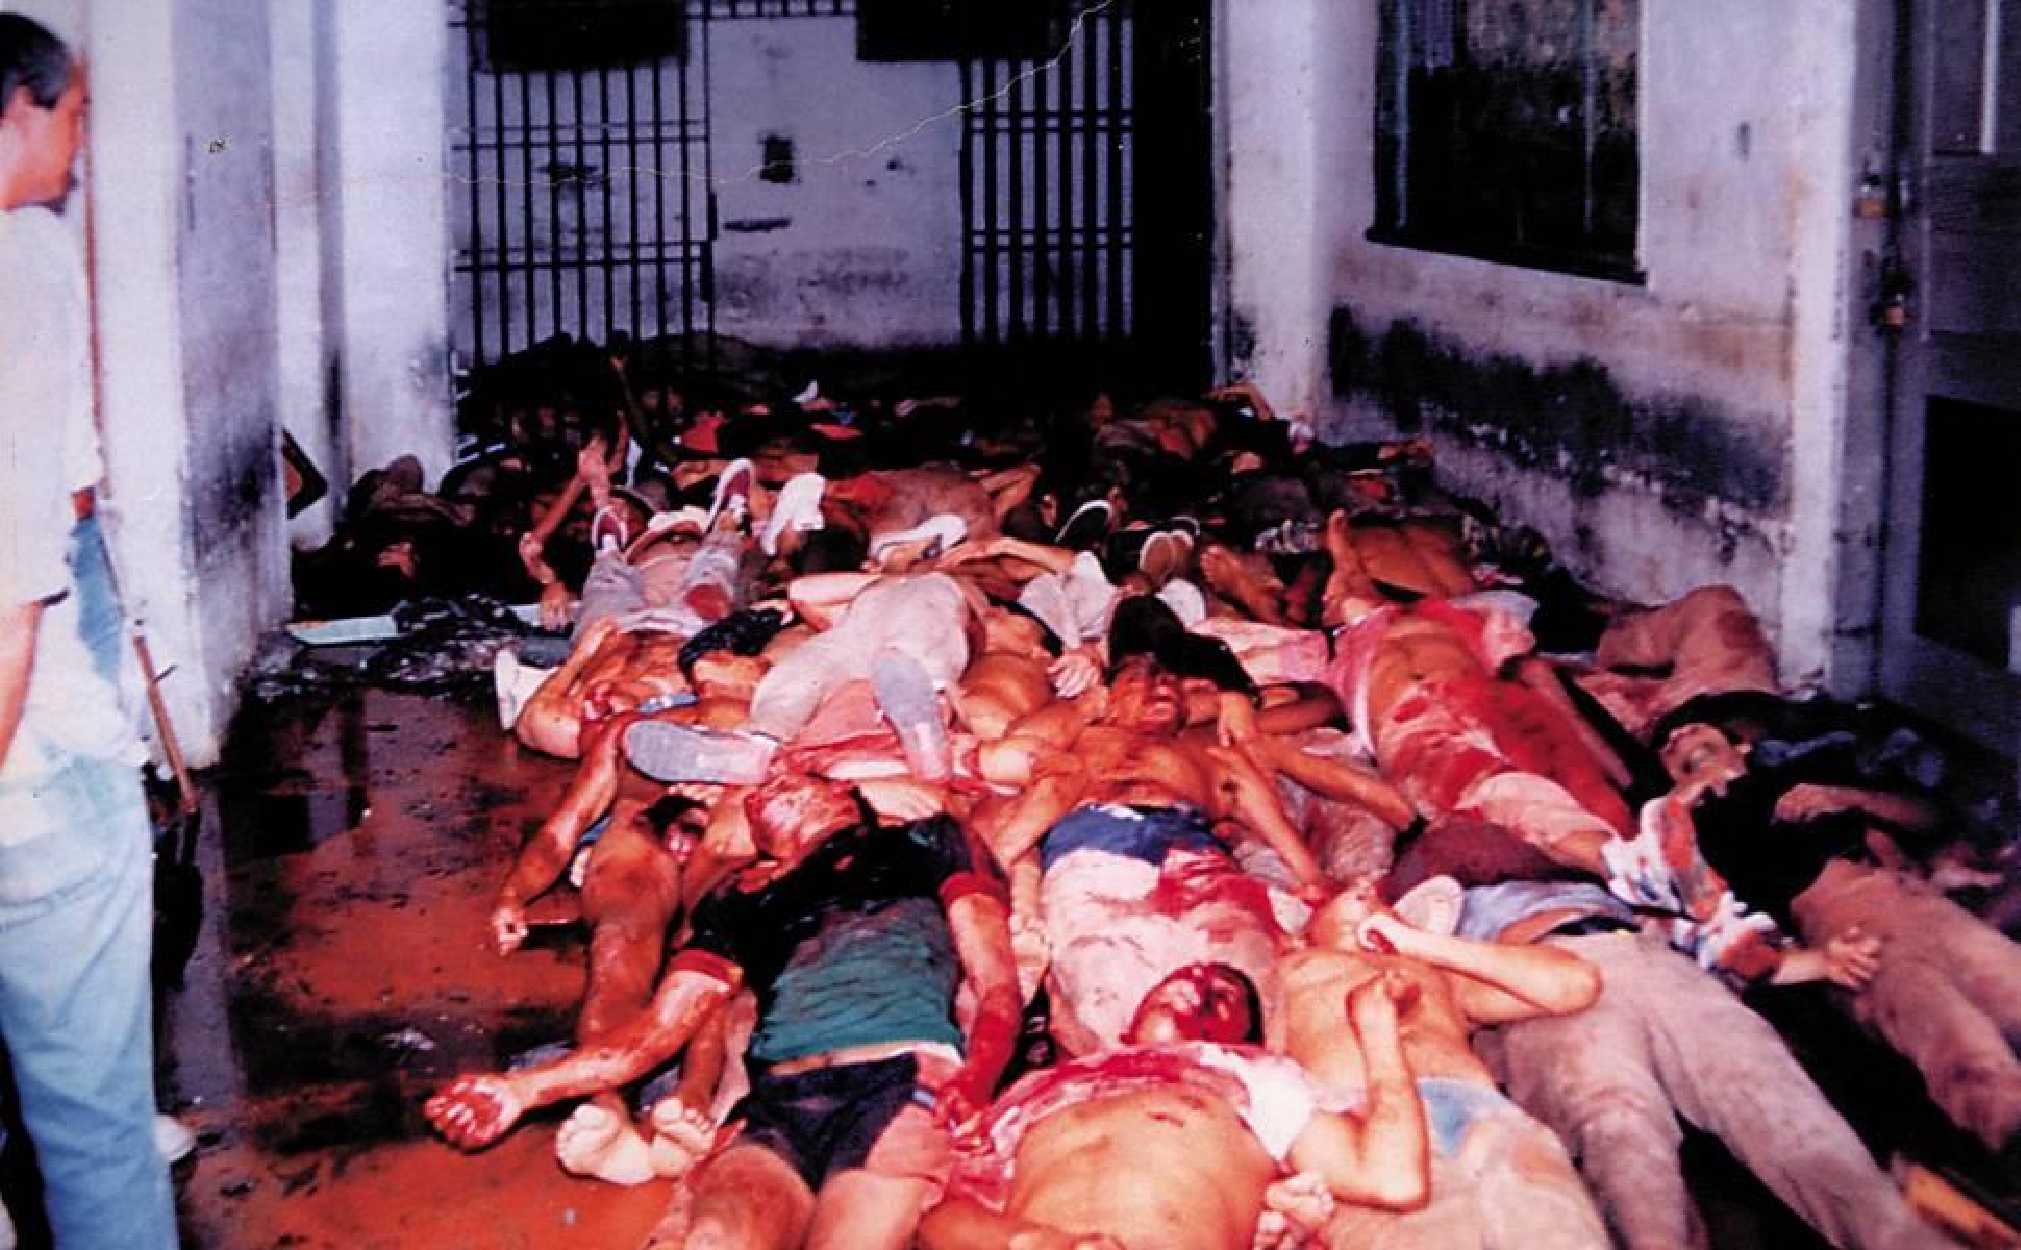
\includegraphics[height = 8cm, width = 1\linewidth]{gfx/fig4}
\caption[Inmates killed by the police in the Carandiru Massacre, 1992]{Inmates killed by the police in the Carandiru Massacre\footnotemark}
\label{fig:fig4}
\end{figure}
\end{center}

\footnotetext{Source: Folha de S\~{a}o Paulo.}

\section{Foundation: After Carandiru}

The Primeiro Comando da Capital was officially founded on 31st August, 1993, by eight detainees\footnote{Namely, Mizael Aparecido da Silva (``Miza''), Wander Eduardo Ferreira (``Cara Gorda'' -- ``Fat Face''), Ant\^{o}nio Carlos Roberto da Paix\~{a}o (``Paix\~{a}o''), Isa\'{i}as Moreira do Nascimento (``Esquisito''  -- ``Weirdo''), Ademar dos Santos (``Da F\'{e}'' -- ``Faith''), Ant\^{o}nio Carlos dos Santos (``Bicho Feio'' -- ``Ugly Beast''), C\'{e}sar Augusto Roris da Silva (``Cesinha'' -- ``Little C\'{e}sar'') and Jos\'{e} M\'{a}rcio Fel\'{i}cio (``Gelei\~{a}o'' -- ``Big Jelly'') \citep[]{folha2006criada}. The inmates are mainly known by their nicknames. \citet[69]{biondi2010junto} notes that there are different versions for the foundation of the PCC, but apparently the prisoners abandoned all of them in favour of the story told by \citet[]{jozino2004cobras}, who published a widely-circulated book in the mid-2000s. \citet[69]{biondi2010junto} also writes that it was not the first time she saw such examples of ``collective amnesia'', when PCC members seem to ``forget'' or downplay certain facts that may cause rife between prisoners.} of the \textit{Casa de Cust\'{o}dia de Taubat\'{e}} (``Taubat\'{e} Custody House''). The jail is located in the countryside of S\~{a}o Paulo \citep[60]{matos2009lado}, and was then considered the safest penitentiary in the state. Nevertheless, as described by William Langewiesche \citep[]{vanityfair2007pcc}, 

\begin{quotation}
Conditions there were atrocious. The prisoners lived locked alone into 160 dark and putrid cells, surviving on filthy slops, defecating into holes they could not flush, and subject to beatings by the guards. They were released into the yards only every few days, and in groups of merely five. Some committed suicide. Most, however, were tough, and managed not only to remain vital, but also to communicate fully from cell to cell.
\end{quotation}

A discussion that allegedly began after a football match was the trigger of a serious fight between inmates. Two prisoners were killed and others were wounded\footnote{The story goes that Gelei\~{a}o broke the neck of a rival gangster on the pitch, in front of all criminals and guards \citep[134]{santos2010dimensao}.}. The eight remaining detainees, fearing a brutal punishment by the warden, decided to swear a public vow of mutual defence. The gang was christened as \textit{Primeiro Comando da Capital}, and is also referred to as \textit{Partido do Crime} (``Criminal Party''), \textit{Fam\'{i}lia} (``Family''), \textit{Quinze} (``Fifteen''), and \textit{15.3.3} (``PCC'' in the Brazilian alphabet) \citep[25]{biondi2010junto}. The group soon published their statute, probably written by Miza. Their constitution, only 16 articles long, lays out the rules members are expected to obey. The statute commands:

\begin{enumerate}
\item Loyalty, respect and solidarity to the Party, above all.
\item The Struggle for liberty, justice and peace.
\item The unity of the Struggle against injustice and oppression inside prisons.
\item The contribution from those who are in liberty to the brothers inside prisons through lawyers, money, help to family members and prison outbreak operations.
\item The respect and solidarity to all members of the Party, so there are no internal conflicts, for he who causes conflicts within the Party, trying to divide the brotherhood will be excluded and shunned from the Party.
\item Never use the Party to solve personal conflicts with outsiders. Because the ideals of the party are above personal conflicts. But the party will always be loyal and supportive to all its members so that they do not suffer any inequality or injustice in external conflicts.
\item He who is in liberty and enjoying a good life, but forgets to contribute to the brothers in jail, will be condemned to death without forgiveness.
\item Members of the Party have to set an example, and for that reason the Party does not allow mugging, rape and extortion within the System.
\item The Party will not tolerate lies, treason, jealousy, greed, misdirection, selfishness and personal interest. It values truth, fidelity, manhood, solidarity and the interest in the common good, because we are one for all and all for one.
\item Every member has to respect the order and discipline of the Party. Each one will be paid accordingly to what he deserves for what he has done. Everyone's opinion will be heard and respected, but the final decision will be made by the founders of the Party.
\item The Primeiro Comando da Capital (PCC) was founded in the year of 1993, in an overwhelming and tireless struggle against oppression and injustice in the concentration camp of the Casa de Cust\'{o}dia (``House of Custody'') of Taubat\'{e}, with the absolute motto ``Liberty, Justice, and Peace''.
\item The Party will not tolerate internal rivalries, disputes for the leadership of the Command, as each member of the Command knows his own role according to his own capability to execute it.
\item We must remain united and organised to avoid a similar or worse massacre as the one which occurred on 2nd October, 1992, when 111 prisoners were cowardly murdered, a massacre that will never be forgotten in the consciousness of the Brazilian society [the Carandiru Massacre]. For we from the Command will change prison practices [that are], inhumane, full of injustices, oppressive, [with] torture and prison massacres.
\item The priority of the Command is to put pressure on the State Government to deactivate the Concentration Camp of House of Custody of Taubat\'{e}, from where the roots of the Command originated, in the middle of such inglorious and atrocious suffering.
\item Emanating from the Central Command of the Capital of the HQ of the State, the simultaneous action directives in all of the State's prison facilities, in a truceless, borderless war until the final victory.
\item The most important of all is that no one will stop us in this struggle, for the seed of the Command has spread to all prison systems of the state and we have managed to structure ourselves outside [of prisons] as well, with many sacrifices and irreparable losses, but we have consolidated ourselves at the state level and in the middle and long run we will consolidate ourselves at the national level. In an alliance with Comando Vermelho (CV) and PCC, we shall revolutionise the country from within prisons and our armed wing will be the terror of the powerful oppressors and tyrants that used the Taubat\'{e} Annex and Bang\'{u} I in Rio de Janeiro as an instrument of vengeance from the society to the creation of monsters.

\vspace{.3cm}

We know our strength and the strength of our Powerful enemies, but we are ready and united, and a united people will never be defeated.

\vspace{.3cm}

LIBERTY! JUSTICE! AND PEACE!

\vspace{.3cm}

PCC Headquarters, First Command of the Capital, in alliance with Comando Vermelho (CV)

\vspace{.3cm}

UNITED WE SHALL WIN!\footnote{The statute was first publish by \citet{folha2001estatutopcc}. Capital letters in the original. To the best of my knowledge, the statute has never been changed or amended.}
\end{enumerate}

The PCC statute performs the three functions of criminal constitutions described by \citet[]{leeson2010criminal}. First, the statute promotes consensus among PCC members by creating common knowledge about what the organisation expects from them and what they can expect of each other. All articles, in this sense, have such function. Second, it also regulates behaviour that, while beneficial to private individuals, may be damaging to the PCC as a group. The fact that criminals cannot invoke the gang to solve personal issues, for instance, is a clear example of that. Whereas the PCC may indeed be used as a mediation tool within and outside prisons \citep[]{dias2009ocupando}, the Command cannot be called to address questions which are \textit{strictly personal}, like a family feud. Finally, the statute mentions what are the punishments for deviations to the expected behaviour individuals are supposed to have after they become members of the cartel. Prisoners who try to ``divide  the  brotherhood'' will be banned from the group and, curiously, those do not finance the gang shall be put to death. Such harsh punishment probably indicates that the organisation has been concerned with expanding his reach since its foundation, what makes collaboration one of the most important tasks for the group members.

%The manner by which individuals join to the gang goes as follows. After being \textit{batizados} (``baptised'') by the cartel\footnote{The baptism usually works like this: an inmate who is already in a PCC-dominated prison (called \textit{primo} -- ``cousin'') can become a full member of the PCC after being formally invited to join the gang by two other \textit{irm\~{a}os} (``brothers''), detainees who are already affiliated with the cartel. If the inmate decides to accept the offer, those two detainees who invited him will be then considered his \textit{padrinhos} (``godfathers'') and take responsibility for future actions of their proteg\'{e}e. Since the process implies costs for the two detainees, they tend to indicate an third inmate only after long periods of friendship. This explains why prisoners may stay as \textit{primos} for years before they are officially accepted in the PCC \citep[210]{biondi2007relacoes}.}, the inmates are called \textit{irm\~{a}os} (``brothers'') and can claim that they belong to the group. Criminals generally address each other as \textit{ladr\~{a}o} (``thief'') regardless of the crime perpetrated by the individual, and although PCC members also use \textit{irm\~{a}os} to refer to each other, the more general term ``thief'' is employed very often. Its meaning, if derogatory, neutral or even complimentary, depends widely on context \citep[]{marques2009crime}. In contrast, police officers, members of rival gangs, and other enemies are called \textit{coisa} (``thing'') or \textit{verme} (``worm'') \citep[169]{dias2011pulverizaccao}. 

%There are three ``political positions'' that a PCC member can occupy, namely \textit{faxinas} (``cleaners''), \textit{pilotos} (``pilots''), and \textit{torres} (``towers'') \citep[110-123]{biondi2010junto}. The first group comprises inmates who work as mediators between prisoners and state institutions, and are also in charge of the cleaning and management of everyday affairs. \textit{Pilotos} are ``spokespeople'' to the inmates, and are democratically elected by the detainees to voice their concerns and represent them in negotiations \citep[1102]{dullo2012biondi}. ``Pilots'' are elected at many different levels, being usually a representatives of the cell, corridor and prison. The role of the \textit{torres} is a bit more difficult to grasp. From what is currently known, the towers are groups of senior inmates who jointly debate and decide (usually by consensus) some of the most serious issues regarding the organisation, such as giving order, solving disputes and ordering punishments. However, PCC members are quite elusive about the meaning and scope of such groups, and so far there is not a single academic research that clarifies under what circunstances the torres are called to act and what tasks they are allowed to perform \citep{biondi2010junto}.

Drauzio Varella, a respected oncologist who served as a volunteer for 13 years at Carandiru\footnote{Varella also wrote a long memoir about inmate life in Carandiru \citep[]{varella1999estaccao}, a text with later became the main source for a successful drama film directed by Hector Babenco. See: \href{http://www.sonyclassics.com/carandiru/}{http://www.sonyclassics.com/carandiru/}. Access:  25th May, 2014.}, mentions how important it is for prisoners to organise themselves, and how effective that social division of labour used to be. In an interview to \citet[]{vanityfair2007pcc}, the doctor said:

\begin{quotation}
Rats who are overcrowded become violent. There have been experiments in the United States to show it. But Carandiru showed that people in those same conditions will organise, and establish rules for their survival. The rules in Carandiru evolved as the prison grew more crowded. They were not written down, but were passed on as understandings. For instance, you had to wash. Every day. And during meal delivery you could not stay in the hallways. For hygiene. Inside the cells, when people were eating, you could not use the toilet. You could not spit. You could not cough. You could not pick your teeth. [\dots] Some of the cell blocks had more than a thousand prisoners. Five, six guys per cell. [\dots] I was so impressed that it was possible in Carandiru for these men to organise in such a way. But, you know, anarchy does not endure in human affairs. And there is no empty space for power in prison.
\end{quotation}

Despite such a high level of organisation and several attempts to mobilise themselves against the public authorities, S\~{a}o Paulo state government used to vehemently deny the groups' own existance \citep[]{bbc2012pcc}. State officials frequently said that there was no such thing as a prison gang in S\~{a}o Paulo, even though a couple of journalists had already collected clear evidence that a criminal organisation had been operating in the penal system \citep[]{jozino2004cobras, souza2007pcc}. In 1996, F\'{a}tima Souza -- an investigative journalist of one the Brazil's main TV channels -- presented the first piece of news where the PCC was presented as an organisation. Unsurprisingly, the government's response quickly dismissed what the journalist had published. In the Souza's words (emphasis mine) \citep[]{obs2007pcc}:

\begin{quotation}
I made a robust piece of news, eight minutes, and we aired it on Band\footnote{Bandeirantes Network, a national broadcasting company based in S\~{a}o Paulo. See: \href{http://www.band.uol.com.br/tv/}{http://www.band.uol.com.br/tv/}. Access:  25th May, 2014.}. For the first time the word ``PCC'' appeared in the scene. The government denied it, obviously. The secretary of prison administration, [Jo\~{a}o] Benedito [de Azevedo] Marques, even spoke to Jovem Pan [radio station] saying I invented such story to gain more points at IBOPE\footnote{IBOPE is the \textit{Instituto Brasileiro de Opini\~{a}o P\'{u}blica e Estat\'{i}stica} (``Brazilian Institute of Public Opinion and Statistics''), a firm that conducts research on media, public opinion and voting intention. It is widely known in Brazil, and its name is often used as a synonym for audience ratings. See: \href{http://www.ibope.com.br/}{http://www.ibope.com.br/}. Access:  26th May, 2014.}, and that what I was talking about a \textit{fiction} not about a \textit{faction}. This made me very angry. My own colleagues were making fun of me: ``So, where is the PCC, are you making news up?'' At the time, the only colleague in the press who took it seriously and decided to know more about it was Josmar\footnote{Josmar Jozino, journalist for the \textit{Di\'{a}rio de S\~{a}o Paulo} (``S\~{a}o Paulo Daily''), author of an important book on PCC \citep[]{jozino2004cobras}.}, which knew how I used to work and that I was not making up a story.
\end{quotation}

For many years there was a strong self-censorship in the public and private media about the existence of the PCC. \citeauthor{jozino2004cobras} (\citeyear{jozino2004cobras}, 143 apud \citeauthor{biondi2010junto}, \citeyear{biondi2010junto}, 74) comments that the editors of the newspaper he used to work

\begin{quotation}
[\dots] banned the use of the acronym PCC, the number $15.3.3$ and the name ``Primeiro Comando da Capital''. The acronym was banned indefinitely from texts, titles, subtitles, headlines or first-page covers. The newspaper should only refer to the PCC as ``criminal faction that dominates the prisons in S\~{a}o Paulo'', or ``criminal group'', or even ``criminal organisation.'' This rule was also extended to the remaining newspapers, magazines and radio and TV networks of the same group, based in Rio de Janeiro\footnote{The \textit{Di\'{a}rio de S\~{a}o Paulo} belongs to the Globo Network, the largest media conglomerate in Latin America. The TV network is the most well-known in Brazil, and the second largest in the world (after the American Broadcasting Company). It presently reaches 99.5\% of the Brazilian population. Any ban adopted by such a large company would surely have a strong impact in the Brazilian public. See: \href{http://redeglobo.globo.com/Portal/institucional/foldereletronico/ingles/g_globo_brasil.html}{http://redeglobo.globo.com/Portal/institucional/foldereletronico/g\_globo\_brasil.html}. Access:  26th May, 2014.}. The acronym CV and ``Comando Vermelho'' was banned.
\end{quotation}

Nevertheless, this false feeling of security did not last for long. A few years after its foundation, the PCC would stage two spectacular series of rebellions in the state, briefly described in \autoref{ch:chap1}. Here I focus on how the PCC organised itself and managed to perform such violent acts.

\section{Consolidation: The Rebellions of 2001 and 2006}

In the end of the 1990s, the PCC progressively expanded their control to other prisons in S\~{a}o Paulo. Apart from the group's own actions, two structural factors collaborated to the growth of the PCC in state prisons \citep[]{adorno2007organized}. First, S\~{a}o Paulo saw a remarkable increase in incarceration rates in the 1990s and 2000s\footnote{See \autoref{fig:fig2}.}. As the total number of detainees went up, the demand for physical and property rights protection in prisons by the inmates also increased which favoured the emergence of a broker and mediator such as the PCC. Also, the precarious conditions of the state jails forced the inmates to develop new ways of coping with scarcity. Thus, having a group which has already devised a set of rules that prisoners can follow in order to maintain order is something of great importance. Second, in an attempt to reduce their influence, several PCC leaderships were transferred to prisons in the countryside, sometimes very far from the capital. Nevertheless, against the government's expectations, instead of isolating the PCC members, the mobsters ended up establishing contact with local criminals, what soon enlarged the \textit{Comando}'s presence in other regions of the state \citep[103]{dias2011pulverizaccao}. 

The rise of the PCC was welcomed by the vast majority of inmates. Anecdotal evidence suggests that S\~{a}o Paulo's prison hierarchies were established mainly through the use of force, and all sorts of conflicts were solved either via physical punishment or by imposing strong humiliations to the individuals \citep[]{adorno1991sistema, ramalho1979mundo}. \citet[4]{negrini2002enjaulado}, himself a detainee in Carandiru prison, shows how common the confrontatios were. In his words,

\begin{quotation}
The scene that unfolded was common. The guards would only interfere after someone was on the floor, stabbed and bleeding. The remaining prisoners formed a large circle, also without interfering. Someone would only leave that [duel] dead or injured and completely demoralised. [\dots] As a result of these fights, prisoners will be respected [and treated] as strong and brave, as leader of their cells, as untouchables. 
\end{quotation}

Acts of violence seemed to be widespread in the penal system, and narratives of fights and physical disputes abounded in the specialised literature on S\~{a}o Paulo's state prisons. But even though physic strength did matter in prisons \citep[]{thompson1980questao, ramalho1979mundo}, there were always exceptions to the rule. Instead of being merely a crude, raw version of Thrasymachus' sentence in Plato's \textit{Republic} -- that ``[\dots] the just is nothing else than the advantage of the stronger''\footnote{See: \href{http://www.perseus.tufts.edu/hopper/text?doc=urn:cts:greekLit:tlg0059.tlg030.perseus-eng1:1.338c}{http://www.perseus.tufts.edu/hopper/text?doc=urn:cts:greekLit:tlg0059.tlg030.perseus-eng1:1.338c}. Access: 28th May, 2014.} (1.338c) -- Brazilian prisons were probably more similiar to the Hobbesian state of nature, where skills and tactics were crucial to survival. Hobbes' famous argument posits that ``[\dots] the weakest has strength enough to kill the strongest, either by secret machination or by confederacy with others that are in the same danger with himself'' \citep[61]{hobbes1985leviathan}. Drauzio Varella confirms Hobbes' insight and affirms that ``[\dots] strength had no role at Carandiru, because people had to sleep. And if you gather 20 guys, even Mike Tyson wouldn't stand a chance'' \citep[]{vanityfair2007pcc}. Since the possibility of temporarily ganging up with other prisoners was always present in jails, the lack of security was pervasive in Brazilian prisons. It affects the weak and the strong alike.

After the PCC started to control the prison system, many inmates claimed that the former chaotic environment was gradually replaced by a sort of \textit{pax mafiosa}, where disputes were solved through PCC tribunals and the use to violence was progressively limited. Commenting on the \textit{Party}, Aldair, an evangelical pastor interviewed by Sacramento \citep[apud][71]{biondi2010junto} told that:

\begin{quotation}
I am not defending crime, but before PCC's existence, prisoners used to suffer very much. They used to suffer because they belonged to different gangs. There used to be much extortion, rape, trivial deaths. But when I knew about the \textit{Partido}, in 88, when I was a pastor\footnote{As pointed by \citet[71]{biondi2010junto}, at that time (2003) there were still conflicting opinions about the PCC's foundation date.} [\dots] I started to observe the way they [PCC members] worked, I saw that the jails had changed. The jails you had to buy\footnote{Aldair refers to the (then) usual practice of paying a fee to other prisoners or gangs to have a place to sleep in one of the overcrowded cells in S\~{a}o Paulo.} nowadays you don't need to buy them anymore, there's no more rape in prison, those trivial deaths don't exist anymore. Thus one can see there had been a change. [\dots] To me, it [the PCC] has only been doing right.
\end{quotation}

As a result, we see that the PCC has successfully reduced homicide rates within the penal system in S\~{a}o Paulo. However, their rise to power was not inevitable. The \textit{Comando} had killed a great number of rival gangsters during its first period of existence \citep[]{passos2013defesa}, and also spent large amounts of money to bribe corrupt police officers and prison staff\footnote{Money was obtained either from the ``taxes'' demanded to prisoners or from crimes (specially bank robberies) perpetrated by its affiliated members on the streets \citep[]{mingardi2007trabalho}.}. From 1999 to 2001, when the PCC was in the process of monopolising the violence within prisons in S\~{a}o Paulo, there was a significant increase in crime rates in the state, including the number of inmate deaths. The graph below displays the number of prisoners killed by other detainees.

\begin{center}
\begin{figure}[bth!]
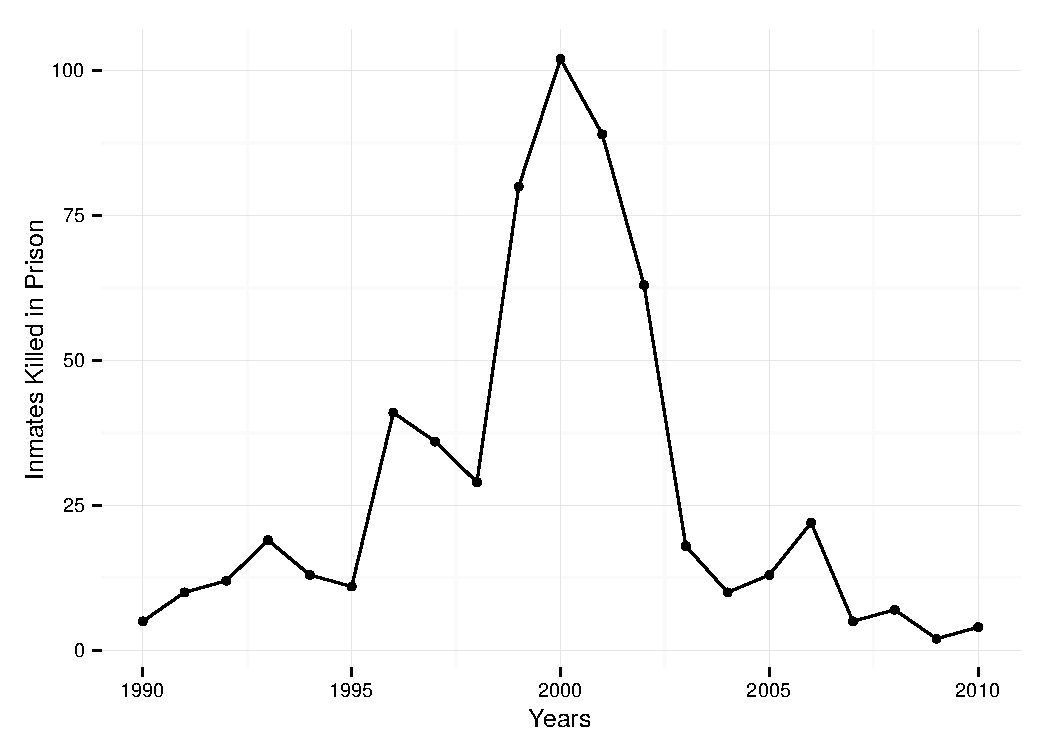
\includegraphics[height = 8cm, width = 1\linewidth]{gfx/fig5}
\caption[Inmates Killed in Prisons (1990--2010)]{Inmates Killed in Prisons (1990--2010)\footnotemark}
\label{fig:fig5}
\end{figure}
\end{center}

The\footnotetext{Source: Own authorship, with data provided by \citep[147]{dias2011pulverizaccao}.} rebellions in February 2001 were a major step in PCC's strategy of dominance. The \textit{Comando} unleashed simultaneous revolts in 29 prisons of the state, coordinating thousands of inmates. On the one hand, this series of attacks made it impossible for the government to deny the existence of the PCC, as it had done before. The rebellions were probable the largest ``publicity stunt'' for the group: at one blow, the PCC made itself both feared by the population and respected by criminals \citep[]{demedo2007}. Rumours go that just after the rebellion of 2001, there were long queues of prisoners asking to join the PCC ranks, and in Carandiru only, hundreds were baptised in a single gathering \citep[401]{dias2013organized}. The PCC had then entered into a virtuous circle: with new members, the \textit{Partido} was able to mobilise an even greater amount of financial and human resources, what would help them to control the remaining prisons in S\~{a}o Paulo. PCC's expansion to other regions was also intensified, and the cartel managed to extend its operations to other Brazilian states and even to other countries\footnote{The cartel has currently consolidated its presence in 22 of the 27 Brazilian states, has recently established itself in Paraguay and in Bolivia, earns about US\$ 60 million a year and plans to fund political campaigns in the next national elections to elect their own representatives \citep[apud][]{veja2013}.}. 

One of the tools that allowed the PCC to articulate such a powerful show of force was the widespread use of mobile phones within jails \citep[]{santos2010dimensao}. Brought by friends or relatives, mobile phones became a necessary tool for PCC members to organise themselves and coordinate actions outside prison walls. The 2001 rebellion started from the Carandiru prison, but it took only a few minutes for the inmates to spread the information to the other prisons via mobile phones \citep[]{terra2001rebeliao}. Although the government had been trying to ban cell phones from jails, corrupt agents still helped to smuggle such devices\footnote{Recently, it was reported that prison guards asked for about 10,000 dollars to smuggle a mobile phone into prison, around 30 minimum wages. See: \href{http://bit.ly/1rjtA3N}{http://bit.ly/1rjtA3N}. Access: 29th May, 2014.}.

As an indirect result of the rebellions in 2001, there was a remarkable change in the PCC's command. In 2001, the cartel was headed by Idemir Carlos Ambr\'{o}sio, nicknamed Sombra (``Shadow''), but no less than 5 months later, he was beaten to death in the same prison where the group had been founded. The leaders then became Gelei\~{a}o (``Big Jelly'') and Cesinha (``Little Ceasar''), two of the original members of the gang. Nevertheless, their rule did not last much longer. Although both criminals were responsible for articulating an important agreement with Rio de Janeiro's largest drug cartel -- the \textit{Comando Vermelho} -- their policies were considered ``too harsh'' to other PCC members, and they were suspected of using the group to increase their power at the expense of others. Moreover, Gelei\~{a}o and Cesinha were in solitary confinement, so it was difficult for them to oversee their subordinates and enforce their orders. The gangsters' wives (Petronilha and Aurinete) were to a large extent responsible for the \textit{Partido} \citep{istoe2013marcola}. 

In 2002, the two women started a feud to decide who would control the main businesses of the PCC. This event indirectly triggered the most significant change of the whole history of the group, when Marcos Willian Herbas Camacho (``Marcola'') become PCC's undisputed leader. Marcola has been the head of the organisation since 2002, and he is widely regarded as the person who modernised the PCC and turned it into the most feared and profitable drug gang in Brazil \citep[]{insight2012pcc}. According to news sources \citep{istoe2013marcola}, Ana Maria Olivatto, Marcola's ex-wife and lawyer, supposedly gave Cesinha's mobile phone number to the police, probably to help Marcola in one of the gang's internal disputes. A few weeks later, Aurinete, Cesinha's wife, killed Marcola's ex-wife. As a retaliation, Marcola gathered support from several PCC members who were unhappy with Gelei\~{a}o and Cesinha and decided to take control over the organisation. Accused of collaborating with the police and with a rival group, Cesinha was brutally murdered a couple of months later \citep[]{folha2006cesinha} and Gelei\~{a}o received a death sentence from the PCC \citep[]{congressoemfoco2006marcola}. Since the mid-2002, Gelei\~{a}o has been in solitary confinement because it is widely believed he will be killed as soon as he moves to a regular cell. With both leaders removed, Marcola was then put at the top of the organisation.

Marcola implemented several important measures just after he became PCC's \textit{capo di tutti capi}. Still in 2002, he decided to incorporate \textit{equality} into PCC's previous motto (``\textit{peace, justice and freedom}'') and dissolved the previous hierarchical structure that had been adopted by the gang since its foundation in 1993 \citep{biondi2010junto}. Consequently, all PCC members can now occupy any position in the organisation and no one -- with the partial exemption of the ``torres'' -- can force any \textit{irm\~{a}o} to do something against his will. Whenever possible, decisions are to be taken by consensus, and all political positions in the PCC are distributed according to the group's specific needs and the availability of ``technical group'' in the gang's ranks. In a certain sense, Marcola modernised the PCC by using the same techniques that nation-states employed to increase their efficiency: civil equality, the attack on privilege, and the creation of careers open to talent \citep[]{hobsbawm2010age}. Therefore, the PCC has become a rational, profit-driven enterprise, in which division of labour, productivity and loyalty to the firm are acknowledged and rewarded. 

This modernisation push can surely be credited to Marcola himself. Marcola is definitely not a regular inmate. An accomplished bank robber and a very skillful manager, Marcola has allegedly read more than 3,000 books since he was imprisoned in the 1990s, maintained a special taste for Nietzsche and Dostoevsky, and usually gives a copy of Sun Tzu's \textit{The Art of War} to every person he trusts \citep[]{epoca2005marcola}. 

Well-cultured and enjoying protection by the PCC itself in S\~{a}o Paulo's maximum security prison (Presidente Venceslau), Marcola has been administering the PCC's rise with great success. Recent footage shows that, using smuggled mobile phones, he closely oversees PCC's deals and alliances\footnote{``S\~{a}o Paulo under Attack'', a TV documentary made by Brazil's second largest broadcasting company (SBT) shows how easy it is for Marcola to pass orders to other PCC members. Link: \href{http://youtu.be/SOSDA-t1lOc}{http://youtu.be/SOSDA-t1lOc} (in Portuguese). Access: 30th May, 2014.}, and regularly discusses PCC's internal affairs with other high-level PCC members even while incarcerated.

\begin{center}
\begin{figure}[bth!]
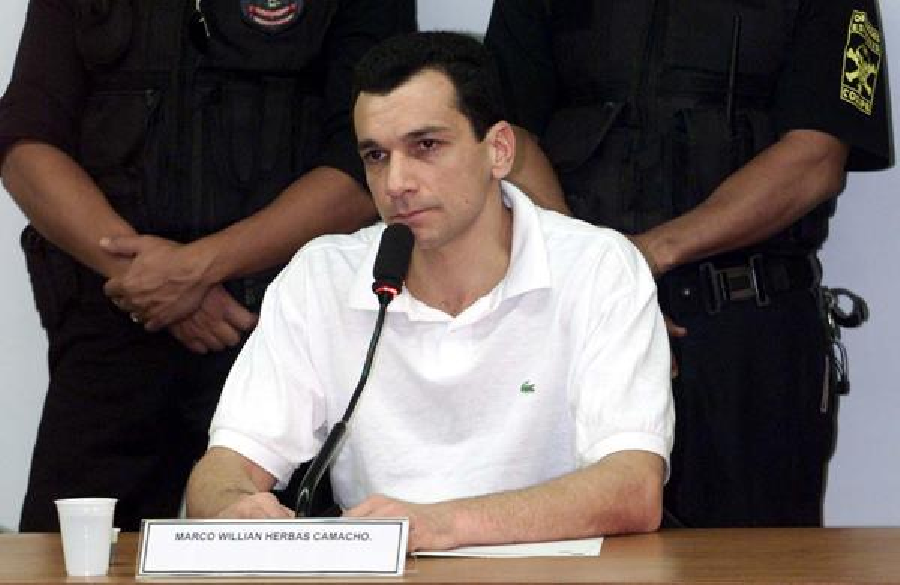
\includegraphics[height = 8cm, width = 1\linewidth]{gfx/fig6}
\caption[Marcola, PCC's leader]{Marcola, PCC's leader\footnotemark}
\label{fig:fig6}
\end{figure}
\end{center}

Marcola was also the mastermind behind the massive rebellions of 2006\footnotetext{Source: Cedoc/RAC.}. From March to July, he coordinated 82 rebellions in prisons in S\~{a}o Paulo and other neighbouring states. The PCC attacked hundreds of civilians, police officers, prison wardens and members of the government \citep[]{folha2006rebeliao, terra2008rebeliao}. It has recently been unveiled that the PCC even had a sophisticated plan to murder the current governor of S\~{a}o Paulo, Geraldo Alckmin, who has been taking a harsher stance against the criminal organisation \citep[]{estadao2013alckmin}. 

The group's terror tactics were ahighly effective against the population, too. During the attacks in May, 2006, schools and universities cancelled their classes, firms dismissed their employees, and all shopping malls were closed. Retail sales in S\~{a}o Paulo, Latin America's richest city, fell about 90\% in the week where most attacks were concentrated (12th t 17th May) \citep[]{uol2006pcc}. More importantly, about 500 people were killed -- including police officers, prison staff and civilians -- in just a few days, a very strong demonstration of force by any standard. From the PCC's viewpoint, the rebellion was a success: its impact was soon felt by the public and the government. For the first time in the group's history, there is plenty of evidence that the state accepted all PCC's demands and decided to go to the negotiation table with the gang. According to the International Human Rights Clinic, the cease-fire was conditional to the promise that the \textit{Tropa de Choque}\footnote{S\~{a}o Paulo's riot police.} would not enter into the penitentiaries, and the granting of additional rights to prisoners\footnote{Stable link: \href{http://bit.ly/1iK4h1i}{http://bit.ly/1iK4h1i}. Access: 2nd June, 2014.}. Two days after an informal meeting with Marcola (15th May 2006), the rebellions stopped \citep{folha2006fimataques}. 

\section{Hegemony: From 2006 to Date}

The attacks of 2006 represent the definitive step in PCC's consolidation process. The \textit{Partido} has successfully institutionalised its power, and to paraphrase the famous Weberian definition (\citeyear{weber1919politik}), the group has attained the monopoly of the legitimate use of physical force [\textit{Gewaltmonopol}] in the prison system. Furthermore, as predicted by theories of state formation, there has been a significant reduction in the number of prison rebellions. \autoref{fig:fig5} shows that the number of inmate deaths has also fallen drastically over the last years. Similarly, the use of symbolic violence, such as the beheading of members of other gangs, has virtually disappeared after 2006 \citep[166]{dias2011pulverizaccao}. 

PCC's monopolisation of violence has also brought changes to the the dynamics of violence in the city. According to several data sources, violence has decreased quickly in the poorest areas of S\~{a}o Paulo. \citet[]{de2010crime} indicates that the new ``crime courts'' deployed by the PCC in the outskirts of S\~{a}o Paulo are perhaps one of the central factors explaining the drop in homicide rates in city over the last two decade. Moreover, such courts could only be fully institutionalised after the PCC had ascended to the position of the legitimate legislative body among a minor, but relevant part of the residents of city suburbs.

We also note a shift in PCC's main financial sources. Whereas in the beginning of the 2000s the group obtained most of its funds via bank robberies and kidnapping, recently the \textit{Comando} has clearly become a drug cartel. It is not a coincidence that the group established itself as a powerful drug gang at the same time it consolidated its power over S\~{a}o Paulo's penal system. Drug dealing is clearly lucrative, but it also demands more bribes to police officers, a high investment on illegal weapons, and low levels of inter-gang violence to have a profitable business in the long. As pointed out by Alba Zaluar, drug traficking ``cannot last without institutional support''\footnote{Stable link: \href{http://bit.ly/1kguPwz}{http://bit.ly/1kguPwz}. Access: 2nd June, 2014.}. The graphs below show how the pattern of violence has changed in S\~{a}o Paulo\footnote{Source: Own authorship. Data provided by \citet[76]{dias2011pulverizaccao}}. 


\begin{center}
\begin{figure}[bth!]
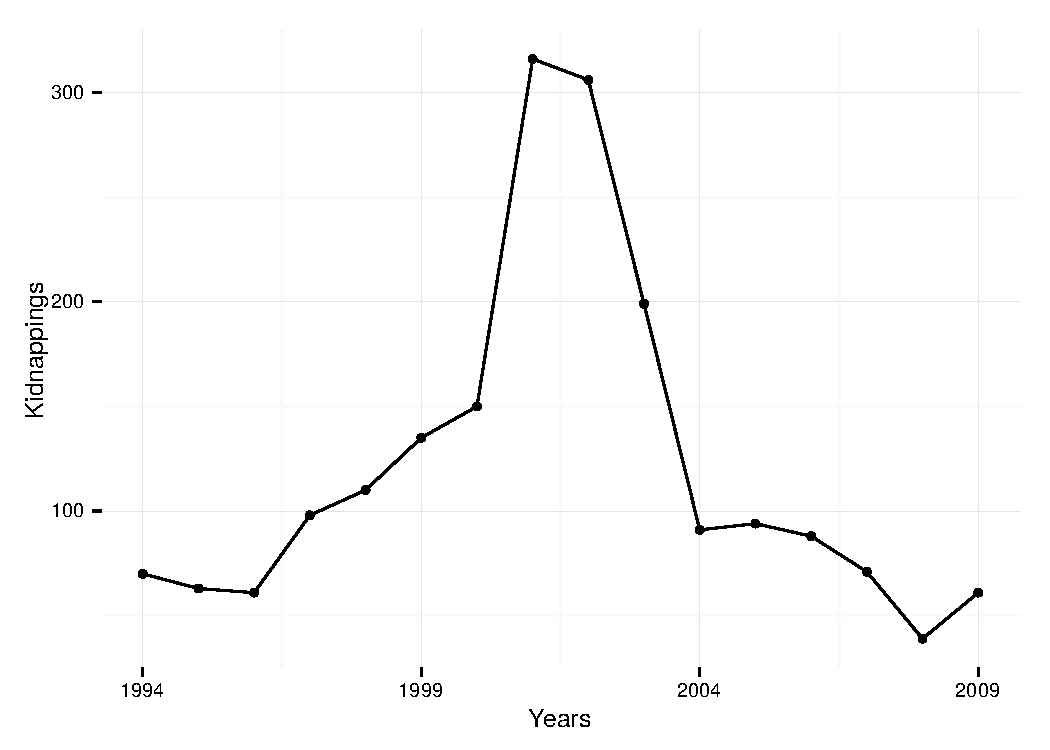
\includegraphics[height = 8cm, width = 1\linewidth]{gfx/fig7}
\caption[Kidnappings in S\~{a}o Paulo (1994--2009)]{Kidnappings in S\~{a}o Paulo (1994--2009)}
\label{fig:fig7}
\end{figure}
\end{center}

\newpage

\begin{center}
\begin{figure}[bth!]
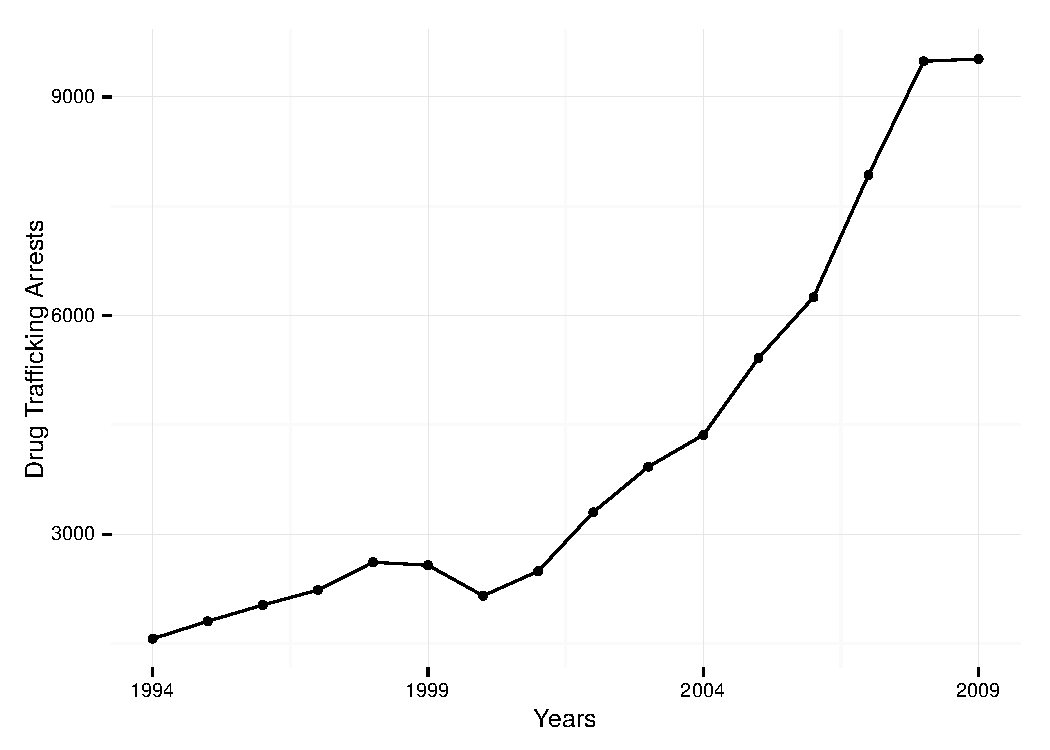
\includegraphics[height = 8cm, width = 1\linewidth]{gfx/fig8}
\caption[Drug Trafficking Arrests in S\~{a}o Paulo (1994--2009)]{Drug Trafficking Arrests in S\~{a}o Paulo (1994--2009)}
\label{fig:fig8}
\end{figure}
\end{center}


In a nutshell, the PCC has established itself as the largest prison gang in S\~{a}o Paulo by successfully devising a long-term strategy. In its initial stage, the group published a clear code of conduct that should be followed by all its members, and emphasised the need for financial support by punishing non-collaborative members to death. Later, the PCC promoted a spectacular demonstration of power that greatly impressed other inmates, the government and the public, therefore increasing their levels of credibility both inside and outside the prison system. During Marcola's leadership, the \textit{Comando} also modernised its practices by having a more inclusive discourse -- which stated that all prisoners should to treated equally -- and professionalised its cadres by adopting a meritocratic selection of members to its political positions. Finally, the PCC has skillfully used different types of threats and violence to eliminate rivals and improve collective action in the incarcerated population.

\section{Recruiting Potential Members}

The manner by which the PCC enlisted members has changed throughout its history. Whether in the beginning the gang used to selected its potential exclusively by their ties with the founding inmates, currently the procedure is much more professional and sophisticated. The first part is the \textit{batismo} (``baptism''). The baptism happens as follows. First, the inmate should already be a resident in a PCC-dominated prison, and show disposition to be engaged in the gang. As in any rationally-motivated enterprise, skillful prisoners are the ones that the PCC aspires to have in its ranks, and the cartel tries to choose only those who have already ``represented''\footnote{Here I tried to stick to the original term, \textit{representado} literally ``represented'', because it can also find an easy translation in English. To ``represent'' is also used with the same meaning in the United States, and the Urban Dictionary defines it as ``Go and be a good example to the others of your group or in your position''. This is precisely the idea conveyed by the PCC's native term. See: \href{http://www.urbandictionary.com/define.php?term=represent}{http://www.urbandictionary.com/define.php?term=represent}. Access:  12th June, 2014.} the criminal underworld in important situations \citep[99]{biondi2007relacoes}. Those detainees are called \textit{primos} (``cousins'') and are already closer to be admitted to the group. 

After this stage, there is what \citet[100]{biondi2007relacoes} aptly call the ``construction of the \textit{irm\~{a}o} (``brother''), how the PCC members are called. This period can last for several months, and it is both an opportunity for the ``cousin'' to show his criminal abilities and for the members to assess the candidate. If the ``cousin'' is deemed fit for the gang, two detainees who are already affiliated with the cartel formally accept him in the PCC. The prisoner can either accept or refuse the invitation.

However, there are costs for both sides if the inmate decides to join the group. The two detainees who invited the new member will be then considered his \textit{padrinhos} (``godfathers''), and should take some responsibility for the future actions of their proteg\'{e}e. Therefore, nominating someone who later makes a mistake is something criminals clearly want to avoid, as punishment can sometimes be harsh \citep[101]{biondi2007relacoes}. Second, the PCC is also in trouble if it accepts members who do not meet the group's high standas. Not only their lack of skills might put in risk the gang's operations -- and thus lead to strong repression by the state -- but bad members are also more likely to miscalculate the effects  of their actions and force the group to engage in unreasonable disputes, both with other gangs and within the PCC itself.


%After being \textit{batizados} (``baptised'') by the cartel\footnote{The baptism usually works like this: an inmate who is already in a PCC-dominated prison (called \textit{primo} -- ``cousin'') can become a full member of the PCC after being formally invited to join the gang by two other \textit{irm\~{a}os} (``brothers''), detainees who are already affiliated with the cartel. If the inmate decides to accept the offer, those two detainees who invited him will be then considered his \textit{padrinhos} (``godfathers'') and take responsibility for future actions of their proteg\'{e}e. Since the process implies costs for the two detainees, they tend to indicate an third inmate only after long periods of friendship. This explains why prisoners may stay as \textit{primos} for years before they are officially accepted in the PCC \citep[210]{biondi2007relacoes}.}, the inmates are called \textit{irm\~{a}os} (``brothers'') and can claim that they belong to the group. Criminals generally address each other as \textit{ladr\~{a}o} (``thief'') regardless of the crime perpetrated by the individual, and although PCC members also use \textit{irm\~{a}os} to refer to each other, the more general term ``thief'' is employed very often. Its meaning, if derogatory, neutral or even complimentary, depends widely on context \citep[]{marques2009crime}. In contrast, police officers, members of rival gangs, and other enemies are called \textit{coisa} (``thing'') or \textit{verme} (``worm'') \citep[169]{dias2011pulverizaccao}. 

%There are three ``political positions'' that a PCC member can occupy, namely \textit{faxinas} (``cleaners''), \textit{pilotos} (``pilots''), and \textit{torres} (``towers'') \citep[110-123]{biondi2010junto}. The first group comprises inmates who work as mediators between prisoners and state institutions, and are also in charge of the cleaning and management of everyday affairs. \textit{Pilotos} are ``spokespeople'' to the inmates, and are democratically elected by the detainees to voice their concerns and represent them in negotiations \citep[1102]{dullo2012biondi}. ``Pilots'' are elected at many different levels, being usually a representatives of the cell, corridor and prison. The role of the \textit{torres} is a bit more difficult to grasp. From what is currently known, the towers are groups of senior inmates who jointly debate and decide (usually by consensus) some of the most serious issues regarding the organisation, such as giving order, solving disputes and ordering punishments. However, PCC members are quite elusive about the meaning and scope of such groups, and so far there is not a single academic research that clarifies under what circunstances the torres are called to act and what tasks they are allowed to perform \citep{biondi2010junto}.

In this sense, two questions remain unanswered. Firstly, if the PCC has managed to control most of the jails in S\~{a}o Paulo, why does not \textit{every inmate} want to be a member of the gang? While it is known that the PCC has a relatively strict admission process, where a new member can only join the group after being nominated by two members, there are many prisoners who do not even \textit{want} to be part of the \textit{Comando}. It has been estimated that 
\textit{less then 3\%} of the inmates in S\~{a}o Paulo have any formal relationship with the PCC\footnote{Although the number seems small, the cartel has about 8,000 members. In comparison, the Mexican Mafia, the biggest prison organisation in the United States, has 150--300 official members \citep[703]{skarbek2011governance}. Thus, the PCC is 53 times larger than \textit{La Eme}  if we use the most conservative estimate.} \citep[]{bbc2013pcc, veja2013crescimentopcc}. \citep[98]{biondi2007relacoes} notes that in provisory detention facilities the number is even smaller, about 1\%. Why are the remaining prisoners not engaged in joining the cartel, if they could have some clear benefits? As far as I know, this large share of the incarcerated population has not been the object of any qualitative study, let alone a model formulation. Would joining the PCC be a dominant strategy, or does an ``independent'' position in a gang-dominated prison also have some benefits?

Another puzzling question is how the PCC manages to select skillful criminals in an environment marked by uncertainty. Lack of trust is also widespread amongst criminals, it is difficult to establish a credible commitment of both parts, non-members and the PCC. Choosing a good member is a much more difficult task for a prison gang than it is for the government or for a firm, since a bad decision can literally be deadly to the the group. Thus, how has the PCC succeeded in choosing its members quite successfully so far?

% Communication in prisons is notably limited, so inmates have strong incentives to fake their credentials, show a different behaviour and try to obtain advantages at the group's expense. 

The next chapters aim to answer those questions. In the following section I develop a simple game-theoretical model to address the issues of individual choice in a PCC-dominating correctional facility. In \autoref{ch:chap5} I use agent-based computational modeling to evaluate the different uses of violence by prison gangs. The model is informed by qualitative data gathered by scholars, as discussed in \hyperlink{page.17}{chapter 2}, and could in theory be generalised and be tested in similar environments. In this sense, my goal here is to formulate two simple, intuitive models that expand the current findings on one of the world's largest prison gangs and provide subsidies for a future general theory of gang violence.

%This is largely in line with theories of state formation. For instance, \citet{buchanan1973defense} argues that a monopoly of violence is better than a free market competition on protection since the monopolist has strong incentives to under-produce violence and allocate those resources elsewhere\footnote{Theoretically, one can say that the underproduction of violence is Pareto superior in a partial equilibrium setting.} The author writes that after a monopoly has been established ``[\dots] resources involved in enforcement may be freed for the  production of alternative goods and services that are positively valued; the taxpayer has additional funds that he may spend on alternative publicly provided or privately marketed goods and services'' \citep[402]{buchanan1973defense}. Those resources have been mainly invested in the enlargement of the group's stake in the drug selling business in S\~{a}o Paulo, and as we have show in \autoref{fig:fig8}, it seems that such strategy has been largely successful.

 % Chapter 3

\cleardoublepage % Empty page before the start of the next part

%------------------------------------------------

\ctparttext{Informed by existing qualitative data on the \textit{Primeiro Comando da Capital}, in the next chapter I develop a simple game-theoretical model to analyse the incentives for a criminal to join a prison gang and how such organisations are able to hire competent criminals under conditions of uncertainty and information asymmetry. Finally, I discuss the findings and point to possible extensions of this research.} % Text on the Part 2 page describing the content in Part 2

\part{A Formal Model of Prison Gang Recruitment} % Second part of the thesis

\chapter{Modeling Prison Gang Recruitment}
\label{ch:chap4}

%----------------------------------------------------------------------------------------

\begin{chapquote}{Diego Gambetta, \textit{Codes of the Underworld}.}
Criminals embody \textnormal{homo \oe conomicus} at his rawest, and they know it.
\end{chapquote}

Criminal games are played for very high stakes \citep[2]{dixit2011game}. In the underworld, rules tend to be enforced by the use of lethal violence, therefore mistakes are rarely tolerated and commitments have notably high exit costs \citep{campana2013cooperation}. Prisons take those situations to the extreme \citep{sykes1958society}. Since prisoners share the same space for long periods of time, their interactions are maximised and the chances of fleeing and escaping retaliation are quite low. Moreover, prisoners have their schedules tightly controlled by correctional officers, what imposes clear limits on the detainees' ability to meet and negotiate \citep[7]{skarbek2014social}. If communication between inmates is limited, they usually have to rely upon costly signals such as acts of brutality or body marks, which are by definition inconvenient for the prisoners \citep[]{gambetta2009codes}.

It is also obvious that prisoners often cannot ask for penal institutions to solve their issues, even if they wanted to. Firstly, the penal system has limited resources, so surveillance is imperfect. There is a very small guarantee that the guards will be able to protect the inmates as well as they should \citep[20]{skarbek2014social}. In places like S\~{a}o Paulo, where prisons are overcrowded and officers are knowingly corrupt \citep[]{darke2013inmate, lemgruber2005brazilian, silveira2007realidade}, this is indeed the normal state of affairs. Secondly, even if the penal authorities were honest, officers may not have information on the illegal activities carried by prisoners, such as drug selling or requests for target killings \citep[]{kauffman1988prison}. Thus, they would be unable to mediate or prevent this sort of conflict. However, being seen as an informer in the prison seriously increases the chances that the inmate will suffer severe retaliations \citep[]{aakerstrom1986outcasts}, so even if the guards would have this kind of information it would be unlikely that inmates would ask them for help. Therefore, in the criminal world one is can usually can count only on oneself, and the choices a prisoner makes have serious consequences. What would then be the best strategy for an inmate to adopt?

As we have seen in this thesis, prison gangs are to a large extent a response to these problems \citep[]{camp1985prison, fleisher2001overview}. Gangs reduce transaction costs, enforce physical and property rights protection, and behave as brokers in correction facilities \citep{buentello1991prison, delisi2004gang, skarbek2011governance}. Nevertheless, prison organisations also have their own interests, and they need to maximise their strength by recruiting prisoners who are the ``most competent'' in the underworld. This is definetely not an easy task. 

In the following pages I present a simple formal model to address this question. My intention here is to devise an analytical framework that might explain a criminal's choice to join a prison gang, and how the organisation reacts to that. I have based my game-theoretical model here upon qualitative evidence from the PCC, either gathered by newspapers or scholars, and tried to stick as closely as possible to the group's own categories and actions.

\section{The Model}

The model consists of two players, a prisoner $P$ and a prison gang leadership $G$\footnote{I use a notation similar to that employed by \cite{lessing2014cddrl}.}. Since the purpose of the present exercise is to evaluate the likelihood of $P$ joining a gang, I shall assume that $G$ is already present in a given prison. Therefore, $G$ moves first, and sets a cost $\tau$ to be paid by the prisoner. This a very common PCC practice: not only the need for financial contributions are specified in the article number 7 of their statute (see page \hyperlink{page.27}{27}), but it has been reported by S\~{a}o Paulo's most important newspaper that PCC members are now asked to pay 50 Reais  (about US\$ 25) per month when in jail, and 500 Reais when free \citep[]{folha2006criada}. Also, PCC members are expect to engage in the group's risky plans, so other important non-monetary costs are also captured by $\tau$. Here I assume that such cost is known by $P$, either because the information is described in the PCC statute (see page \hyperlink{page.24}{24}), or because it has been disseminated by the inmates in a PCC-controlled prison.

The prisoner can either comply ($C$) and bear the costs $\tau$, or defect and be independent in the prison ($D$). $G$ plays next, and after assessing if $P$ meets its criteria, chooses whether to accept ($A$) or reject ($R$) the new member, and payoffs are realised.

\begin{figure}[htp]
\centering
\begin{tikzpicture}	[solid node/.style={fill,circle,inner sep=1.5pt}, hollow node/.style={fill,circle,inner sep=1pt}, scale=1.5,font=\footnotesize]
\tikzstyle{level 1}=[level distance=15mm,sibling distance=40mm]
\tikzstyle{level 2}=[level distance=15mm,sibling distance=30mm]
\tikzstyle{level 3}=[level distance=15mm,sibling distance=20mm]
\node (root)[solid node, label=above:{$G$}] {}  
    child {node (a1) [solid node, label=right:{$P$}] {} 
    child{node[hollow node, label=below:{$\left(0,0\right)$}]{} edge from parent node[left]{$D$}}
   child{node(3)[solid node, label=right:{$G$}]{} 
    child{node(4)[hollow node, label=below:{$\left(0,0\right)$}]{} edge from parent node[left]{$R$}}
    child{node(5)[hollow node, label=below:{$\left(1,1\right)$}]{} edge from parent node[right]{$A$}}
    edge from parent node[right]{$C$}
	}
};
\node [draw=none, shift={(.3cm,-1cm)}] (root) {$\tau$};
	\end{tikzpicture}
\caption{Gang Prisoner Acceptance}
\end{figure}

Let $S$ be a measure of the gang's capacity to ameliorate prison conditions. I assume that the true value of $S$ is known to both the prisoner and the gang, what implies that the players have a perfect understanding of how $G$ can help the $P$ by providing both public and club goods. The assumption is reasonable. The benefits given by the PCC, such as protection and financial assistance, are widely advertised in prisons and they are precisely the reason why inmates would join the group \citep{folha2012pendrive}.

Let $s \sim U \left[0,1\right]$ be a series of skills that are useful for prison life. These can be physical strength or other abilities such as strategic thinking, technical expertise or a dense personal network. The prisoner knows his own value $s_P$, whereas $G$ only knows that that $s$ follows a uniform distribution. The utility of $s_P$ increases monotonically, as more skills are always preferred to less. 

The expected net utility can thus be represented as a simple difference between the benefit ($b$) of being in a prison gang and the benefit of remaining independent. As we have seen above, the costs for a prisoner to be in a gang are higher are also positive, since the prisoner has to pay a monthly monetary tax to the PCC and also follow the group's rules and take part in their actions. 

\begin{align}
b_P\left(s,1\right) - b_P\left(s,0\right) &\geq 0\\
c_P\left(s,1\right) - c_P\left(s,0\right) &\geq 0
\end{align}

Nevertheless, there exists a value $\overline{s}$ such that

\begin{align}
b_P\left(s,1\right) - c_P\left(s,1\right) &\leq b_P\left(s,0\right) - c_P\left(s,0\right)
\end{align}

If $s_P \geq \overline{s}$. That is, above a given value of $s$ it is interesting for a prisoner to ``go it alone.''\footnote{Obviously, the opposite is true whether $s_P < \overline{s}$.} If $P$ has enough skills to survive in prison by himself, $P$ might ponder if it is really profitable for him to join any kind of group. For prisoners who are below this threshold, becoming a member is a dominant position. The benefits are therefore $S_P$ = $1$ if the prisoner decides to comply with the gang's cost $\tau$ and the group accepts him as new member ($A_P$ = $C$ and $A_G$ = $A$). In contrast, $S_P$ = $0$ when $A_P$ = $D$ or $A_G$ = $R$, that is, when the prisoner defects or the gang refuses to have in its ranks. 

As for the gang, there is a low threshold $\underline{s}$ under which any member acceptance implies more costs than benefits to the gang. Any prisoner below this value is likely to become a burden to $G$ since he will not be competent enough to fulfil the tasks demanded by the group, and might lower the collective welfare by increasing other members' chances of being punished by the police. Therefore, there exists $\underline{s} \in \left[0, 1\right]$ such that

\begin{align}
b_G\left(s,1\right) - c_G\left(s,1\right) &\leq b_G\left(s,0\right) - c_G\left(s,0\right)
\end{align}

When $s\leq \underline{s}$, and reverse situation when $s \geq \underline{s}$. $G$ will only choose a member that maximises its utility (a high value of $s$), and reject every prisoner it sees as unfit for the job due to his lack of competence in criminal activities.

\subsection{Perfect Information Game}

Assuming that the prisoner and the game have access to complete, there are three possible equilibria to this game. Whether $s_P \in \left[0, \underline{s} \right]$, $P$ will comply and try join the group ($C$), while $G$ will refuse him ($R$). If $s_P \in \left[\underline{s}, \overline{s} \right]$, the equilibrium is ($C$, $A$), in which $P$ joins the group and $G$ accepts him. Finally, if $s_P \in \left[\overline{s}, 1 \right]$ the equilibrium is ($D$, $A$), and $P$ will remain alone. 

This situation would be valid if $G$ could easily assess the qualities of every potential member. While prison gangs do their best to obtain credible information on the convicts, it is likely that a perfect information game would only be a good approximation to the facts in a very selected number of cases. It is true that prison records provide a reliable source of information on individuals, and gangs often have access to those data via inmates and sometimes even prison staff members \citep[]{gambetta2009codes}. Not only this is a long, costly task, but may not be feasible in some circumstances. High security prisons makes this comprehensive evaluation process virtually impossible. In such environment, the gang cannot be completely sure of the inmate's past behaviour and present intentions, and since interactions between a potential gang member and their ``godfathers in crime'' (see page \hyperlink{page.38}{38}) are relatively few, criminals have difficulties to advertise their credentials to the gang. Recruitment with perfect information is therefore unlikely to happen.

In this regard, I now discuss the recruitment process of a prison gang under conditions of information asymmetry. This is a more realistic assumption, and PCC's history confirms its plausibility. The gang's requirement that every prospective member should receive the approval of two ``brothers'' (current members) before joining the gang is a proof that the gang needs to cross-check information before taking a decision. Thus, the \textit{informants} play a crucial role in PCC's recruitment process, what is indeed expected since an inmate's commitment to the gang is for life. Also, informants have strong incentives to provide reliable information to the PCC, simply because they are held accountable for future actions of their ``godson''. Bad selection choices can not only cost him prestige, but to the extreme lead to severe punishments as fines and expulsion from the group. 

\subsection{Imperfect Information Game}

The next game has the same two players of the previous one, a prisoner $P$ and a prison gang $G$. However, I add a third figure that does not take any action in the game \textit{per se}, but is of extreme importance to the model: the \textit{informer} ($I$). Here, $I$ represents the current PCC member who is in charge of assessing the criminal qualities of a potential candidate. While $I$ has several reasons to provide credible information to the PCC, he can also incur in errors and make wrong judgements about a prisoner's abilities. The information about the prisoner can thus be ($T$) or false ($F$)\footnote{By false I do not imply that wrong information given by $I$ is intentionally manipulated. It can be merely the result of miscalculations, and the term here has no pejorative meaning.}.

To reiterate, the game goes as follows.

\begin{enumerate}
\item Nature chooses the skills of the prisoner $P$, with $s \sim U[0,1]$.
\item The gang leader chooses $t^*$.
\item The prisoner decides if apply or not to the gang. If not, the game ends. If yes, the game follows to the next stage.
\item The gang leader then decides to accept or reject the join proposal. The game ends.
\end{enumerate}

In the present model, I assume that the gang will decide whether it accepts the candidate or not based upon his additional productivity. Therefore, the gang will add a new member if and only if

\begin{align}
\alpha \left( n + 1 \right) \geq \alpha \left(n\right)
\end{align}

Where $\alpha$ is the productivity function and $n$ is the current number of members in the gang. We assume thereafter that exists a number of prisoners that optimises $\alpha(n)$, and we denote it as $\alpha^*$.\footnote{Notice further that the productivity can be expressed by a simple function that has limit $1$ when $n \rightarrow \infty$ and limit $0$ when $n \rightarrow 0$. We assume that this function has a maxima in $n^*$ as well. An example could be $(an)^\frac{b}{n}$, for parameters $a$ and $b$ given.}

The game can be solved via backward induction. The prisoner applies when

\begin{align}
U_P [Comply] \geq U_P [Defect]
\end{align}

The utility of joining is equal to

\begin{align}
\alpha (n+1) s - \tau
\end{align}

Where $\alpha (n+1)$ is the marginal productivity of the new member to the gang, $s$ is the skill of the prisoner and $\tau$ is the fee (monetary and non-monetary) imposed by $G$ on $P$. The prisoner's utility for not joining the gang is simply $s$, which is $P$'s individual ability to survive in prison.

We can then expand the equations as

\begin{equation}
\begin{split}
\alpha (n+1) s - \tau &\geq s\\
[\alpha (n+1) -1] s &\geq \tau\\
s \geq \frac{\tau}{\alpha (n+1) -1} & = s^*(\tau)
\end{split}
\end{equation}

All prisoners with $s \geq s^*(\tau)$ will try to enter the gang. Notice that

\begin{align}
\frac{ds^*(\tau)}{d\tau} = \frac{1}{\alpha (n+1) -1} > 0
\end{align}

Thus, the proportion of prisoners that intend to join the gang shrinks as the leadership rises the fee. In such scenario, $G$ can choose qualified candidates only by increasing the entry barriers. 

Let us now consider that $\tau = \underline{\tau} + t$, where $\underline{\tau}$ is an exogenous cost of joining the gang. To illustrate this situation, imagine that police forces might initiate a crackdown on the prison gang, or that there is a dispute between two different gangs in the same jail. In such scenario, $t$ is the share of the cost that $G$ is imposes in the selection process. The idea is to raise the level of its members, since more skills are needed. $G$ will choose a value of $\tau$ that maximises its revenues and skills. This is given by

\begin{align}
\alpha (n(s^*(\underline{\tau} + t))) \times (1-s^*(\underline{\tau} +t)) \times E(s^*(\underline{\tau} + t))
\end{align}

In which the first part of the equation is the effect caused by the productivity parameter, the second part is the proportion of prisoners that are accepted in the gang and the third the expected productivity of the gang as a whole. Furthermore, as the number of members is always decided by criteria of optimise the productivity $\alpha(n)$, we can without loss of generality change it by $\alpha^*$. Thus, the gang optimises the ex-post utility by maximise the following equation

\begin{equation}
\begin{split}
\max_{t \geq 0} \{ \alpha^* \times (1-s^*(\underline{\tau} +t)) \times E(s^*(\underline{\tau} + t)) \} \\
s^*(t) = \frac{1}{3}
\end{split}
\end{equation}

And solving for $t$ we have that

\begin{equation}
\begin{split}
t^* = \frac{1}{3}(\alpha^*-1) - \underline{\tau}
\end{split}
\end{equation}

And therefore, the duple $t^*$ and $s^*(t^*)$ solves the game for the Gang and the Prisoner, respectively.

This equilibrium has interesting qualitative properties:\\

\noindent 
1) All prisoners with $$ s \geq s^*  = \frac{\underline{\tau} + t^* }{\alpha (n + 1) - 1}$$

Will join the prison gang $G$.\\

\noindent 
2) $t^* = 0$, when the exogenous shocks are high\\

\noindent
3) $t^* > 0$ when there are many prisoners trying to join $G$, or then $\underline{\tau}$ is low. When a high number of prisoners are willing to join the prison gang, it can be implied that low-skilled inmates will also apply and get the spot.\\

\noindent
4) $n^*$ maximises the ex-post benefit for the gang. The reason is that, given that $t*$ had already been chosen, the only preoccupation for the gang is its productivity increase. As long as the new member $P$ can rise $G$'s productivity levels, the gang will accept him.\\

\noindent
5) $t^*$ maximises the ex-ante utility for the gang. The reasoning behind it is that the gang can control the admission of prisoners by selecting only inmates with high values of $s*$.\\

Now, consider the situation when we add the informant. The informant acts as a probability of find out the true value of $s$ of a given applicant. Let this probability be denoted by $\pi$, when the complement means that the information is wrong.

The time-line for the second game follows below.

\begin{enumerate}
\item Nature chooses the skills of the prisoner $P$, with $s \sim U[0,1]$.
\item The gang leader chooses $t^*$.
\item The prisoner decides if apply or not to the gang. If not, the game ends. If yes, the game follows to the next stage.
\item With probability $\pi$ the gang leader finds out the true type of the prisoner. With probability $1-\pi$ the gang leader does not find it.
\item Finally, the gang leader then decides to accept or reject the join proposal.
\end{enumerate}

Adding this new feature the the previous game empowers the gang leader by giving him a better screen process, where he can combine fees and a selection upon the revealing of the quality parameter by the informant.

Solving the game backwards we have that the gang accepts an offer, ex-post the choice of $t$ whenever

\begin{align}
\alpha (n+1)S + \alpha (n+1) \left[\pi s + (1-\pi) E[s*|t] \right] \geq \alpha (n)S
\end{align}

Where $S$ is the sum of the abilities of all current gang members. Solving this equation we have that the gang accepts ex-post the new member when

\begin{align}
s \geq \frac{S}{\pi} \left[\dfrac{\alpha(n)-\alpha(n+1)}{\alpha(n+1)}\right] - \dfrac{1-\pi}{\pi}\left[\dfrac{1-s^*(t)^2}{2}\right] = s^{**}
\end{align}

This equation means that there will be a new limit, $s^{**}$ that, upon the information of the productivity of the prisoner, the gang decides by imposing a higher threshold. This means that $s^{**} > s^*(t)$. The qualitative difference that this will generate is that the gang now can select more skilled prisoners without having to raise the fees $t$. 

In the sequence, the prisoner ask to join the gang if and only if

\begin{equation}
\begin{split}
U_P[Comply] &\geq U_P[Defect]\\
\alpha (n + 1) s - \tau &\geq s \\
s \geq \frac{\underline{\tau}+t}{\alpha (n+1) - 1} &= s^*(t)
\end{split}
\end{equation}

Which is the same as in the previous model. Finally, the ex-ante optimum for the gang will be to set the fees at zero. This because when there is informants inside the process we have that the ex-ante value that the gang maximizes is equals to 

\begin{equation}
\begin{split}
\max_{t \geq 0} \{ \alpha^* \times (\pi(1-s^{**})\int_{s^{**}}^1 \sigma d\sigma + (1-\pi)(s^{**}-s^{*})\int_{s^{*}}^{s^{**}} \sigma d\sigma ) \}
\end{split}
\end{equation}

And optimising in $t$ this expression leads us to 

\begin{align}
t = \left(-\frac{s^{**}}{3} - \underline{\tau} \right) (\alpha^*-1)
\end{align}

And as $t<0$, $t^*=0$ for all parameters, as long as $s^{**}>s^*$.

For the model above, we have the following qualitative properties:

\noindent
1) Information minimises the use of entry barriers by the prison gang;\\

\noindent
2) The quality of the information ($\pi$) provider by the informer $I$ also matters. We see that $\pi$ has a positive impact on $s**$, as $\frac{ds**}{d\pi} > 0$. In a nutshell, it is easy to observe that the more (and better) information available, the more precise the screening process is;\\

\noindent
3) In the present model, the proportion of prisoners remains the same;\\

\noindent
4) However, the difference we observe here is that the gang has now a much more qualified cadre. If $G$ is capable of extracting good, reliable information, it has a significant impact on the abilities of the selected members.

\subsection{Comparison between Models}

The first and more important different between models 1 and 2 is that in the latter the selection process is notably more sophisticated than in the earlier one. The use of information, here designed by $\pi$, helps the gang to choose more qualified members to its ranks.

When we reach the limit satisfaction, that is when $\pi \rightarrow 1$ (when the gang's information of the given prisoner is precise and sufficient), the revenue for the gang is clearly maximised. In a nutshell, for a prison gang information is a very necessary good, certainly crucial for it to recruit the correct prisoner\footnote{The true role of information may be distorted in these conclusions, but note that $\pi$ also changes the second threshold $s^{**}$. This makes information the key to the last result.}.

In the first model, one may observe that $t^* \geq 0$, whereas in the second one $t^*=0$. This is a result of information, which is enough to deter unskilled prisoners from entering the gang.

Interestingly, not only $G$ has a benefit increase when information is added to the model. For $P$, adding information to the selection process eliminates the cost $t^*$, thus reducing the loss for the inmate.

Another interesting point is that such result holds for general $\alpha^*$ values as long as we consider that $\alpha(n)$ has those characteristics assumed in the text. If we assume that $\alpha$ reaches a point where it starts to generate benefits lower than $1$, some prisoners will prefer to ``go it alone'' and not join the prison group. Obviously, the most skilled prisoners will be these ones that shall run alone and the others may free ride, as they are less skilled and can free ride in the group's productivity.

Finally, if we consider the possibility of a lower threshold $\underline{s}$ under which the gang prefers to refuse a prospective member, if $s^* < \underline{s}$, there is the possibility that the gang is indifferent for that choice. In the informer's equilibrium, there is a $\pi$ probability that the inmates will get caught by a third party (the police forces or a rival gang in our example), and shall not join the gang. This measure avoids the fact that the gang leadership would become weaker.



%%%%%%%%%%%%%%%%%% The following paragraph is now useless, but it might
%I also present a slight change to the model. Instead of having a continuous distribution of $s_P$ (a set of $P$'s criminal skills), in this part I have three discrete categories in this parameter, so that $s$ = $\{0,1,2\}$. This classification also mirrors the manner by which the PCC refers to prisoners in general, as a ``thing'' (\textit{coisa}, former member of a rival gang or untrustworthy criminals), a ``thief'' (\textit{ladr\~{a}o}, a competent criminal), or a ``rascal'' (\textit{malandro}, criminals who are either very smart or want to take advantage of other inmates.) Such categorisation maintains the same idea presented before, that there exists a value where $s$ is too low for $G$ to accept $P$ as a member, and that there is high threshold of $s$ which creates incentives for $P$ to not join the prison gang. However, the classification into categories makes the model easier to understand, since it simplifies the calculations without loss of generality.
 % Chapter 4
\chapter{Discussion}
\label{ch:chap5}

%----------------------------------------------------------------------------------------

\begin{chapquote}{Thomas Paine, \textit{A Dissertation on the First Principles of Government}.}
He that would make his own liberty secure, must guard even his enemy from oppression; for if he violates this duty, he establishes a precedent that will reach to himself.
\end{chapquote}


The present thesis discussed how the \textit{Primeiro Comando da Capital}, a S\~{a}o Paulo-based prison gang, was able to centralise power and extend its influence to around 90\% of its native state's penal system \citep[]{veja2013}. Recently, the PCC's reach has crossed S\~{a}o Paulo's borders, and it was reported that the cartel has established itself in 22 of Brazil's 27 states, and has even been involved in illegal activities in Bolivia and Paraguay \citep[]{bbc2013pcc}. The PCC has also allegedly been responsible for a remarkable reduction in homicide rates both within and outside the prison system. This is largely in line with theories of state formation. For instance, \citet{buchanan1973defense} argues that a monopoly of violence is better than a free market competition on protection since the monopolist has strong incentives to under-produce violence and allocate those resources elsewhere\footnote{Theoretically, one can say that the underproduction of violence is Pareto superior in a partial equilibrium setting.}. The author writes that after a monopoly has been established ``[\dots] resources involved in enforcement may be freed for the  production of alternative goods and services that are positively valued; the taxpayer has additional funds that he may spend on alternative publicly provided or privately marketed goods and services'' \citep[402]{buchanan1973defense}. Those resources have been mainly invested in the enlargement of the group's stake in the drug selling business in S\~{a}o Paulo, and as we have show in \autoref{fig:fig8}, it seems that such strategy has been largely successful. In this regard, the PCC operates more or less like a ``pseudo-state'' in Brazil's penal system, and seriously undermines the official authority at its very core: the right to punish and protect the social contract \citep[]{hobbes1985leviathan,weber1919politik}.

The rise of the PCC is a good example of unintended consequences of public policies. Whereas the government hoped that its zero-tolerance programme would reduce crime in S\~{a}o Paulo notably violent state, it has fostered the expansion of a much more significant threat to public security, a highly organised and powerful prison gang. Needless to say, the PCC currently represents a much more dangerous threat to public security than the myriad of relatively petty criminals that used to be in charge of S\~{a}o Paulo's illegal markets. In this case, Milton Friedman's famous criticism of public policies seems unfortunately correct. ``One of the great mistakes'', he said in a TV interview with Richard Heffner in 1975, ``is to judge policies and programmes by their intentions rather than their results.''\footnote{The interview can be seen at \href{http://youtu.be/ImMgZHbeb4Q}{http://youtu.be/ImMgZHbeb4Q}. Access: 15th June, 2014.} In this sense, the mass incarceration policy cannot be claimed successful. As Fr\'{e}d\'{e}ric Bastiat insightfully noted more than 150 years ago, every law or institution produces not only effects that are \textit{seen}, but also effects that are \textit{unseen}, which emerge only subsequently \citep[]{bastiat1995selected}. The difference between a good legislator and a bad one is precisely such ability to foresee such unexpected results of public policies; and in S\~{a}o Paulo they were not.

Interestingly, the PCC was able to monopolise power in the penal system having only a fraction of the inmate population in its ranks. The group remains quite small, although its force has increased significantly over the last years. The puzzle I tried to address in this thesis concerns precisely the recruitment process employed by the group. If the PCC offers so many advantages to its members, and it has clear expansionary intents, why is not every detainee part of the gang? Those questions, as obvious as they may seem, had never been addressed by the specialised literature.  Therefore, albeit very modestly, this thesis collaborates to our current understanding of prison gangs and their selection criteria, and also sheds some light on what are the individual incentives to join such criminal groups.

The model has three important findings. First, it shows that a prison gang uses the value of its initial costs as a first selection method, since only skillful prisoners will be able to comply with the gang's demands if the costs are too high. Although useful, this procedure generates costs for both the prisoner and the gang. For the prisoner, it is necessary to spend long periods of time to display all abilities required by the gang, what may lead to an increasing lack of interest for the criminal. The gang also has to bear costs, since the process of establishing and enforcing a high threshold demands considerable human and financial resources from the group. In order to reduce such gang costs, the group can make use of informers. With an informer, the gang can keep a lower entry cost, thus attracting a large pool of applicants while still being able to select competent candidates for the job. 

Second, there are cases in which joining a prison gang is not the best option for an inmate. When the detainee has enough skills to endure prison conditions by himself, he might be better off if he decides to ``go it alone'' and devote his ability exclusively to his own survival. If a prison gang decides to lower its threshold to admit a higher number of members, a competent criminal will have its individual benefit reduced. Since the collective goods provided by the gang would be divided amongst several detainees, his net benefit will be lower than in the previous stage, where the selection process was stricter. However, the gang can eliminate this loss by raising the bar for admission, so that qualified criminals will only share the collective goods with those who can contribute to the group's welfare as much as they do. At its early stages, the PCC indeed followed such strategy in order to maintain the group cohesive enough to carry risky actions without losing highly-skilled members. After the group had already secured its dominance, it was then able to open its ranks to less skilled members and proceed with its model of ``careers open to talent'' (see page \hyperlink{page.33}{33}).

Third, the models confirms the idea that the prison gang is not only a ``school of crime'', but perhaps most importantly, a highly effective screening device \citep[]{gambetta2009codes}. If a given prisoner knows that the admission to a certain gang is difficult to obtain, as soon as he manages to join the gang he can identify peers who are at least as skillful (and trustworthy) as he is. Therefore, prison gang membership solves one of the most critical issues of the criminal underworld, that of \textit{peer identification}. If a prison gang's admission process is deemed as satisfactory by the prisoners, if an inmate joins the gang he sends a signal that only true criminals could afford, thus dramatically reducing the chances that he might be a snitch. This also has the benefit of reducing violence between criminals, as they do not have to constantly ``test'' each others' integrity or to use violence as a communicative means to express one's toughness. Prison gangs thereby increase the welfare of the inmates by providing an extremely valuable public good: reliable information.

Two policy implications can be derived from the findings discussed above. One important suggestion is that states should reduce the total amount of benefits that prison gangs can offer to its members. The most evident manner by which this can be done is by improving prison conditions. For instance, reducing overcrowding in prisons would decrease violence between inmates by decreasing the likelihood of violence disputes for scarce resources such as food, health care and individual space within the cells, all things that are currently being distributed by the PCC in S\~{a}o Paulo \citep[]{dias2009ocupando}. Moreover, if the state is able to reduce police abuse it will lower the need for a crucial public good provided by prison gangs: protection. The more states care about prisons conditions, the less necessary prison gangs are.

Also, the present dissertation questions the recent mass incarceration policy implemented in the state of S\~{a}o Paulo. Such policy has caused devastating effects to the poor population, who has repeatedly been the main victim of both institutional and criminal violence. In this sense, this thesis shows the urge for a discussion on the hidden but persistent channels by which inequality has been perpetuated in the Brazil. 

Finally, it should also be noted that this study can be expanded in several ways. The model shown here was based upon information gathered on the workings of the PCC, and it has to be tested with data from other prison gangs in order to give it external validity. Moreover, due to serious lack of data on the topic, I was not able to incorporate the state dimension into the model. By including corrupt prison officers and weak public institutions to our formal analysis one could make the model even more realistic and derive more robust predictions from subsequent findings. It would lead to a better-informed discussion on the efficiency of the public institutions in Brazil's recent history, and maybe shed some light on the dark side of country's current democratic regime.















%In mathematics, physics and biology, computational models have long been an important method in the researchers' toolbox \citep[71]{box2008oxford}. The increase in computing power over the last decades has allowed for otherwise intractable problems to be solved via simulation. For instance, the advent of Markov Chain Monte Carlo techniques -- implemented by Gibbs sampling or the Metropolis-Hastings algorithm \citep[]{gelman2013bayesian} -- has helped to solve multi-dimensional integrals present in Bayesian analysis, and they were largely responsible for the growing adoption of Bayesian statistics in a vast number of academic fields \citep[]{mcgrayne2011theory}. 

%Agent-based models (ABMs), in this sense, present a new set of possibilities to researchers in general and to political scientists in particular \citep[]{kollman2006computational}. Agent-based models are composed by a set of autonomous, interacting computational objects, known as agents, whose behaviour is rule based \citep[2]{de2014agent}. Agents can be individuals, firms, governments, institutions, or any other category researchers want to analyse. Networks, identities and learning mechanisms can also be embedded in ABMs, thus making the models apt for testing non-linear, path-dependency dynamics in complex systems \citep[3]{bhavnani2004agent}. ABMs have been seen as a ``revolutionary tool'' for the social sciences \citep[]{Bankes14052002}: several social phenomena can be modeled as non-equilibrium, dynamic settings, and scholars can simulate social processes and carry out "experiments" that would otherwise be impossible \citep[]{davidsson2002agent}. 

%\Citet[2--6]{de2014agent} point out that ABMs have six important capabilities: 1) ABMs allow researchers to link behavioural rules to aggregate patterns, be they equilibria or complex patterns; 2) ABMs enable the inclusion of geographic and social space at multiple levels of resolution; 3) ABMs have the capacity to include multiple processes simultaneously; 4) ABMs can include heterogeneity not only in location, beliefs, information, and ability, but also in learning rules, perspectives, mental models, behavioural repertoires , and cognitive framing; 5) ABMs prove capable of producing messy contingent outcomes and a range of phenomena: randomness, equilibria both static and distributional, patterns and complexity, and the complex outcomes can vary in their amount and type of path dependency; and 6) analysis of ABMs tends to focus on outcome robustness, i.e., whether the system can keep doing what it needs to do as opposed to the existence and efficiency of equilibria. To this list we should add two other advantages of ABMs that are particularly relevant for the present research. ABMs can present results in a clear, simple way. Simulation graphs convey the same information contained in game-theoretical mathematical proofs, but have a much more intuitive interpretation. Also, AMBs give us the opportunity to test mechanisms that are difficult to observe due to the inherently secretive and dangerous nature of organised crime. ABMs are therefore the research method of choice for evaluating our hypotheses.

%To the best of my knowledge, there is not a single paper discussing the PCC which employs formal or computational methods. Thus far, no generalisable set of propositions using the PCC as an example has ever been formulated, and this thesis aims to fill this gap. In the following sections I present the a model to analyse individual choices in a prison environment, and evaluate some comparative statics of the model's parameters. % Chapter 5
%\include{Chapters/Chapter06} % Discussion

%----------------------------------------------------------------------------------------
%	THESIS CONTENT - APPENDICES
%----------------------------------------------------------------------------------------

\appendix

\part{Appendix} % New part of the thesis for the appendix

% Appendix A

\chapter{Appendix}
\label{sec:appendix}

%-----------------------------------------------------------------------------------\

\noindent
1) R code for \autoref{fig:fig2}.

{\footnotesize
\begin{verbatim}
# Create the data set
# Sources: http://bit.ly/1rImlPE and http://bit.ly/1ixhY8z

years <- seq(2000,2013)
inmates.brazil <- c(232755, 233859, 239345, 308304, 336358, 361402,
                    401236, 422373, 451429, 473626, 496251, 514582,
                    548003, 574023)
inmates.saopaulo <- c(92186, 98822, 109535, 123932, 131764, 138116,
                      144430, 149310, 154696,163915, 170916, 180059,
                      190818, 203681)
df <- data.frame(years, inmates.brazil, inmates.saopaulo)

# Plot the graph

require("ggplot2")
require("scales")

ggplot(df) + geom_line(aes(years, inmates.brazil), lty = 1) + 
  geom_point(aes(years, inmates.brazil), size = 2) +  
  geom_line(aes(years, inmates.saopaulo), lty = 2) +
  geom_point(aes(years, inmates.saopaulo), size = 2) + 
  scale_x_continuous("Years", breaks=c(2000,2003,2006,2009,2012)) +
  scale_y_continuous("Number of Inmates", labels = comma) +
  annotate("text", 2010.5, 460000, label = "Brazil") +
  annotate("text", 2010.5, 130000, label = "Sao Paulo") +
  theme_minimal()
\end{verbatim}
}

\newpage

\noindent
2) R code for \autoref{fig:fig3}.

{\footnotesize
\begin{verbatim}
# Create the data set
# Source: http://bit.ly/Sg7qjB

year <- seq(2000, 2007)
homicides <- c(5979, 5990, 5435, 5016, 3846, 2784, 2312, 1311)
df <- data.frame(year, homicides)

# Plot the graph

require("ggplot2")

ggplot(df) + geom_point(aes(year, homicides), size = 2) + 
  geom_line(aes(year, homicides), lty = 1) +
  xlab("Year") + ylab("Homicides") + theme_minimal()
\end{verbatim}
}

\noindent
3) R code for \autoref{fig:fig5}

{\footnotesize
\begin{verbatim}
# Create the data set
# Source: Dias (2011, 147)

years <- seq(1990,2010)
inmates.deaths <- c(5, 10, 12, 19, 13, 11, 41, 36, 29, 80,
                    102, 89, 63, 18, 10, 13, 22, 5, 7, 2, 4)

df <- data.frame(years, inmates.deaths)

# Plot the graph

require("ggplot2")

ggplot(df) + geom_point(aes(years, inmates.deaths), size = 2) + 
  geom_line(aes(years, inmates.deaths), lty = 1) +
  xlab("Years") +
  ylab("Inmates Killed in Prison") +
  theme_minimal()
\end{verbatim}
}

\newpage

\noindent
4) R code for \autoref{fig:fig7}

{\footnotesize
\begin{verbatim}
# Create the data set
# Source: Dias (2011, 76)

years <- seq(1994,2009)
kidnappings <- c(70, 63, 61, 98, 110, 135, 150, 316,
                 306, 199, 91, 94, 88, 71, 39, 61)
df <- data.frame(years, kidnappings)

# Plot the graph

require("ggplot2")
require("scales")

ggplot(df) + geom_line(aes(years, kidnappings), lty = 1) +
  geom_point(aes(years, kidnappings), size = 2) +
  scale_y_continuous("Kidnappings", breaks=c(100, 200, 300)) + 
  scale_x_continuous("Years", breaks=c(1994, 1999, 2004, 2009)) +
  theme_minimal()

\end{verbatim}
}

\noindent
5) R code for \autoref{fig:fig8}

{\footnotesize
\begin{verbatim}
# Create the data set
# Source: Dias (2011, 76)

years <- seq(1994,2009)
drug.trafficking <- c(1564, 1804, 2027, 2233, 2614, 2573, 2154, 2491,
                      3300, 3924, 4361, 5415, 6250, 7931, 9490, 9521)
df <- data.frame(years, drug.trafficking)

# Plot the graph

require("ggplot2")
require("scales")

ggplot(df) + geom_line(aes(years, drug.trafficking), lty = 1) + 
  geom_point(aes(years, drug.trafficking), size = 2) +  
  scale_y_continuous("Drug Trafficking Arrests", breaks=c(3000, 6000, 9000)) + 
  scale_x_continuous("Years", breaks=c(1994, 1999, 2004, 2009)) +
  theme_minimal()

\end{verbatim}
}
 % Appendix A
%\include{Chapters/Chapter0B} % Appendix B - empty template

%----------------------------------------------------------------------------------------
%	POST-CONTENT THESIS PAGES
%----------------------------------------------------------------------------------------

\cleardoublepage% Bibliography

\label{app:bibliography} % Reference the bibliography elsewhere with \autoref{app:bibliography}

\manualmark
\markboth{\spacedlowsmallcaps{\bibname}}{\spacedlowsmallcaps{\bibname}} 
\refstepcounter{dummy}

\addtocontents{toc}{\protect\vspace{\beforebibskip}} % Place the bibliography slightly below the rest of the document content in the table of contents
\addcontentsline{toc}{chapter}{\tocEntry{\bibname}}

\bibliographystyle{agsm2}

\bibliography{Bibliography} % Bibliography
\cleardoublepage% Declaration

\refstepcounter{dummy}
\pdfbookmark[0]{Declaration}{declaration} % Bookmark name visible in a PDF viewer

\chapter*{Declaration} % Declaration section text

\thispagestyle{empty}

 
I hereby declare that

\begin{enumerate}
\item except where due acknowledgement has been made, the work is that of the author alone;
\item the work has not been submitted previously, in whole or in part, to qualify for any other academic award;
\item the content of the thesis is the result of work which has been carried out since the official commencement date of the approved research program;
\item any editorial work, paid or unpaid, carried out by a third party is acknowledged;
\item ethics procedures and guidelines have been followed.
\end{enumerate}

\bigskip
 
%\noindent\textit{\myLocation, \myTime}

\smallskip

\begin{flushright}
\begin{tabular}{m{6cm}}
\\ \hline
\centering Danilo Alves Mendes Freire\\Geneva, 16th June 2014
\end{tabular}
\end{flushright}
 % Declaration

%----------------------------------------------------------------------------------------

\end{document}
